\documentclass[12pt]{article}
\usepackage[utf8]{inputenc}
\usepackage{physics}
\usepackage[margin=1in]{geometry}
\usepackage{graphicx}
\usepackage[english]{babel}
\usepackage{mathabx}
\linespread{1.5}
%\fontfamily{ptm}\selectfont
\usepackage{mathptmx}
\usepackage{dsfont}
\usepackage{amsmath}
\usepackage{caption, threeparttable}
\captionsetup{labelfont = sc, textfont = it}

%\usepackage[style=ieee-alphabetic]{biblatex}
\usepackage[
backend=biber,
style=numeric,
sorting=none
]{biblatex}
\addbibresource{BIB.bib} %Imports bibliography file



\title{Choosing Ferromagnetic Alloys for JMRAM Spintronic Transistors}
\author{Author: Nikolaos Palamidas \\\\ Supervisor: Professor Mark van Schilfgaarde\\Fourth Year MSci Project 7CCP4000 \\King's College London}
\date{March 2017}





\begin{document}

\maketitle
\clearpage
\thispagestyle{plain}
\begin{center}
    
    \vspace{0.9cm}
    \textbf{Abstract} 
   \\
   A preliminary mathematical treatment of metallic solids is explored in detail, and its involvement in self-consistent computational methods. The values acquired from these simulations, contribute to understanding many important magnetic and electrical properties of ferromagnetic insulating alloys, which are essential to the theoretical development of spintronic transistors. Through these computational results it is found that magnetisation of the alloys may be quenched significantly by introduction of Copper, but which in turn produces more scattering for both majority and minority spin carriers, and an appropriate balance between these two effects is found. 
\end{center}
\clearpage
\tableofcontents
\clearpage

\section{Introduction}

Global power consumption is continuously increasing, a large portion of which is due to computers and electronic devices. Moore’s law predicts that the number of transistors on a circuit board doubles every two years (since 1971), and while we continue to develop smaller, faster and more efficient transistors, the power consumption is still too high\cite{mram}. This is due mainly to the lack of progress, using roughly the same circuit technology. Currently, the random-access memory(RAM), used in most personal computers is Dynamic RAM (DRAM). DRAM uses a capacitor like transistor that stores logic states by the amount of charge stored on plates. While this method is cheap and easy to produce, DRAM faces many problems. Firstly, DRAM is volatile memory, so if bit states are not changed for an extended period of time, or if power to the DRAM is lost, the capacitor discharges and memory is lost. For this reason, new technologies must be developed, and there is great hope in the field of Spintronics\cite{fundapp}. This technology uses the intrinsic angular momentum properties of electrons to store bit logic states. A relatively heavily tested spintronic transistor is the magnetoresistive RAM(MRAM). Two ferromagnetic plates are constructed adjacent to each other, one with a fixed magnetisation direction, and the other with parallel or antiparallel magnetisation, to be flipped by the application of an external magnetic field. This setup is referred to as a magnetic tunnelling junction(MTJ).  The current passing through these layers will encounter a low or high resistance depending on the relative parallel or antiparallel magnetisation configuration of the layers. While the MRAM is more efficient and a lot of research\cite{mram} has been done, it is still inefficient and slow. We require a faster memory switching, especially in the potential advent of quantum computing. 
\\This report focuses on the theoretical development of superconducting MRAM, also known as JMRAM. It is physically like the MRAM, but now the MTJ is sandwiched between superconducting layers, and the ferromagnetic layer is also electrically insulating.  Now the physics of the magnetoresistance is still applicable but now to supercurrents (currents that flow without dissipation), which allows for fast information transfer. By use of the Josephson effect\cite{josephson}, the superconducting cooper pairs\cite{BCS} quantum tunnel through the acquire a phase when moving through the ferromagnetic insulating layer. For fast switching, we require the magnetisation of the free layer to be reduced. We also require the property that the layers have a small magnetostriction to reduce scattering. A calculation of the Curie temperature must also be carried out to indicate under which temperatures the layers stay ferromagnetic.
\\
Constructing these MTJs with different alloy configurations and testing them all experimentally is very time-consuming, expensive, and labour intensive. We look to computational simulations using solid state physics to predict properties of different alloy configurations, without the need for any experimental investigation. In this report, the theory of Linear Muffin-Tin Orbitals (LMTOs) developed by O.K. Andersen \cite{andersen} is exploited to provide a basis set to describe the electronic structure in metal alloys. The LMTO basis set is used in the self-consistent Density Functional theory (DFT) introduced by Hohenberg and Kohn \cite{inhom}, to construct the ground state properties of the alloy. A Green’s function approach to calculate physical observables is used, particularly the use of the Bloch spectral function, which plots the bands of the alloy. Random alloys simulation requires the use of the coherent potential approximation(CPA)\cite{drchal}, which uses the configurational average of the Green's function to calculate observabled, to account for the random order in the system. All these methods are contained in the ‘lmgf’ code in the QUESTAAL suite \cite{ques}.
\\
By application of these computational methods to predict electronic structure properties of different alloy configurations, the aim of the report is to choose an ideal alloy configuration, applicable for JMRAM transistor technologies.

\section{Density Functional Theory}

\subsection{The Kohn-Sham Equation}
The Hohenberg-Kohn theorems form the backbone of density functional theory (DFT) \cite{inhom}. This theory is to exactly describe any many body system. It can be show very easily \cite{martin}, that the ground state electron density $n_0(r)$, once found, uniquely determines the external(full) potential of the interacting system of electrons, whatever it may be. The second crucial idea, is that the energy of the system is a functional of the electron density i.e. $E[n(r)]$. By varying n(r), and one can determine the ground state density and therefore ground state energy $E_0[n_0(r)]$.
We can write the energy functional in terms of the external potential, the kinetic energy and the electron electron interaction term. It has to be said that all of these equations are in respect to some interacting reference frame.
\begin{equation} \label{2.1} \tag{2.1}
E[n]=\int V\textsubscript{ext}(r)n(r)d^3r + T[n] + V_\textsubscript{ee}[n]
\end{equation}
where 
\begin{equation} \label{2.2} \tag{2.2}
T=\sum_{i} \bra{\Psi_i}-\frac{\hbar^2}{2m}\nabla ^2 \ket{\Psi_i} 
\end{equation}
\begin{equation} \label{2.3} \tag{2.3}
n(r)=\sum_{i} | \Psi_i(r) |^2 
\end{equation}

Here T is the kinetic term, and V\textsubscript{ee} is the potential term containing all electron-electron interactions (more involved than Hartree potential). Now we suppose a non-interacting frame in which to do our calculations. We create a sort of 'fake' augmented Hamiltonian, potential and basis. These are H\textsubscript{s}, V\textsubscript{s}, and $\psi$\textsubscript{i}. The s subscript is for Sham, because these values are used in the Kohn-Sham equations \cite{inhom}. Now we can rewrite the Schrodinger equation for the non interacting frame of N electrons as follows.
\begin{equation} \label{2.4} \tag{2.4}
H_s\psi_i = \sum_{i=1}^{N} [-\frac{\hbar^2}{2m}\nabla_i ^2 + V_s(r_i)] \psi_i \qquad n(r)=\sum_{i=1}^{N} |\psi_i|^2 
\end{equation}

Of course it has to be said that $\psi_i$ is not exactly the single electron wavefunction, in the same way that H\textsubscript{s} is not exactly the full many body Hamiltonian and $V_s \neq V\textsubscript{ext}$. Instead the interactions are absorbed into the augmented Sham values. The sham kinetic energy will be
\begin{equation} \label{2.5} \tag{2.5}
T_s[n]=\sum_{i=1}^{N} \bra{\psi_i}-\frac{\hbar^2}{2m}\nabla^2\ket{\psi_i}
\end{equation}

For the Kohn-Sham equation, we take the augmented $T_[n]s$ to be the real and exact $T[n]$ for the many body system. Of course something needs to balance this out as the interaction component needs to be absorbed in another term, which is called the exchange-correlation energy $E_X_C[n]$. Let us expand the electron-electron interaction more formally into the standard Hartee-Fock potential and the remaining contribution (origins in electron exchange and correlation) $\xi_{ee}$.
\begin{equation} \label{2.6} \tag{2.6}
V_e_e[n] =V_{hartree}+V_{unknown}=\frac{1}{2}\int \int \frac{n(r)n(r')}{|r-r'|} + \xi_{ee}
\end{equation}


Now let us define the exchange correlation in terms of something we know, namely the full many body energy (in the interacting frame) made up of the kinetic and potential terms. On the RHS we have the sham kinetic energy, the classical electron electron repulsion, and have the exchange correlation at the end as a sort of 'sponge' for any interaction components that might be needed to describe the many-body system fully. Upon imposing that $T_s=T$
\begin{equation} \label{2.6} \tag{2.7}
E[n]_{total}=T[n]+V_e_e[n] = T_s[n] + \frac{1}{2}\int \int \frac{n(r)n(r')}{|r-r'|}d^3 r' + E_X_C[n]
\end{equation}
And with simple substitution of (2.7) leads to the fundamental equation
\begin{equation} \label{2.7} \tag{2.8}
E_X_C[n]=T[n] -T_s[n] + \xi_{ee}[n]
\end{equation}

This last equation is an important result as it intuitively shows us what the exchange correlation energy means. It can be thought of as the difference in the real kinetic energy of the whole system and the Sham kinetic energy term of the non interacting system. We know that the interacting electrons are in a potential V\textsubscript{ext}(r), but what auxiliary potential could the non-interacting electrons be in? This shall be called the effective potential $V_e_f_f[n]$. We wish to apply the variational principle to the energy in the interacting $E_i[n]$ and non interacting frame $E_n_i[n]$ upon changing the electron density:
\begin{equation} \label{2.8} \tag{2.9}
E_i=\int V_e_x_tn(r)d^3r + \frac{1}{2}\int \int \frac{n(r)n(r')}{|r-r'|}d^3 r' + T_s[n]+E_X_C[n]
\end{equation}
\begin{equation} \label{2.9} \tag{2.10}
E_n_i[n]= \int V_{eff} n(r)d^3r + T_s[n]
\end{equation}

Now we apply the variational principle to both quantities. 
\begin{equation} \label{2.10} \tag{2.11}
\frac{\delta E_i[n]}{\delta n} = V_{ext}(r) + \int \frac{2n(r')}{|r-r'|}d^3r'  +\frac{\delta T_s[n]}{\delta n} + \frac{\delta E_X_C[n]}{\delta n}
\end{equation}
\begin{equation} \label{2.11} \tag{2.12}
\frac{\delta E_n_i[n]}{\delta n}= V_e_f_f(r) + \frac{\delta T_s[n]}{\delta n}
\end{equation}

Equating the two quantities above we obtain the effective potential in terms of the external potential.
\begin{equation} \label{2.12} \tag{2.13}
V_e_f_f(r)=V_e_x_t(r)  +\int \frac{2n(r')}{|r-r'|}d^3r' + \frac{\delta E_X_C[n]}{\delta n}
\end{equation}

So to summarise, in the real interacting frame the electrons act in  V\textsubscript{ext}(r) and in the auxiliary non interacting frame the electrons act in some $V_e_f_f[n]$ to be determined.

The full Kohn-Sham equation is just an modification to the full Schrodinger equation to include the terms discussed.
\begin{equation} \label{2.12} \tag{2.14}
H_s \psi_i (r) = (-\frac{\hbar^2}{2m}\nabla^2 +V_e_f_f(r) ) \psi_i (r) = \epsilon_i \psi_i (r)
\end{equation}

\subsection{Self-consistent Energy Evaluation}

DFT is a computational method, and to use the variational principle to obtain a self consistent ground state energy, there must be some sort of code loop until self-consistency is reached. So we start with some initial electron density $n_{in}(r)$ and use (2.12) to calculate an effective input potential $V_{in}(r)$. Solving (2.12) gives a generated input wavefunction $\psi_{in}(r)$, which can then be used in (2.4) to calculate an output density $n_{out}(r)$. If $n_{out}(r)=n_{in}(r)$ (to some reasonable degree of accuracy) then self consistency has been reached and the ground state density has been found. If not then we make $n_{out}(r)$ the new $n_{in}(r)$ and iterate the procedure. The final density can now be used to calculate observables like energy.

\subsection{L(S)DA}

The Local spin density approximation (LSDA) is a candidate for the E\textsubscript{XC}. For a simple system with no spin polarisation the local density approximation(LDA) is used instead. While there are many approaches to the functional, the most succesful is that of the homogeneous electron gas (HEG or Jellium).\cite{inhom}\cite{martin}
We define that
$$E_X_C[n(r)]=\int n(r) \varepsilon_X_C[n(r)] dr$$
From the equation it is clear that the $\varepsilon$ is an energy density. L(S)DA is the name given to a whole set of methods where the exchange correlation energy per particle $\varepsilon_X_C$ is uniquely determined by the electron density at a given position n(r), so that $\varepsilon_X_C[n(r)]$.
In the case of a polarised system of majority and minority (up and down) spins, we must use the electron density for each, forming the basis of Local Spin Density Approximation (LSDA):

$$E_X_C[n_\uparrow(r),n_\downarrow(r)]=\int n(r) \varepsilon_X_C[n_\uparrow(r),n_\downarrow(r)] dr$$


The exchange correlation is split into exchange and correlation density terms $\varepsilon_X_C[n(r)]=\varepsilon_X[n(r)]+\varepsilon_C[n(r)]$.
We use HEG exchange and correlation energies to compute $\varepsilon_X_C$. Of course we are not dealing with a uniform/homogeneous electron gas, but a molecule, but what we will assume is that for a given n(r) density, the exchange density is the same for the HEG and the molecule. Even in this HEG, the correlation density is still a problem, and no analytical derivation has been found. It is calculated in \cite{martin} and \cite{exc} that $\varepsilon_X[n(r)]=-\frac{3}{4}\bigg(\frac{6}{\pi}n(r)\bigg)^\frac{1}{3}$ and $\varepsilon_C[n(r)]$ is approximated for different situations.

\clearpage
\section{Muffin Tin Orbital method}%-------------------------------------------------------------------------------
\subsection{Treatment of Metallic lattices}

The potential of a lattice is in general, a very complex mathematical object. To analyse the structure and compute important quantities, we must understand the nature of the delocalised electronic wavefunction throughout the entire lattice potential. For a simple case such as a 2D infinite potential well with one electron, the wavefunction can be found very easily without any complex mathematics. We must simplify the potential problem such that carrying out density functional theory calculations is viable and not so taxing. We start by assuming that each atom is a point charge, and located at position $\vec{R}$. To simplify the problem, we assume that the potential $V(\vec{r})$ is spherically symmetric, i.e. V(r). At the sphere boundary r=s\textsubscript{R}, the potential becomes flat, and remains flat (some constant potential V\textsubscript{0}) between the different atomic lattice sites, which we shall refer to as the interstitial. This is the basic assumption behind the Muffin Tin Orbital approximation (MTO). 
\\
The problem is simplified further by enlarging the spherically symmetric Wigner-Seitz(space filling) sphere potentials till they overlap slightly. In this way the interstitial becomes negligible and it's contribution is neglected. This is called the Atomic Sphere Approximation (ASA)\cite{gunn} and replaces the problem with an integral over all space and all Wigner-Seitz spheres, with complete neglect for the interstitial electron kinetic energy E-V\textsubscript{0}. 
\\
Now to analyse the Schrodinger equation for the ASA, which will be as follows. Let the radius of a muffin tin orbital centred at R be denoted as $s_R$ (generally the R subscript shall refer to the value located at the atomic site where r=R) and the interstitial as I. From here onwards, the standard unit convention of $\hbar=1$ $m=1/2$ and $e^2=2$ is used such that $\hbar^2/2m=1$.
\begin{equation} \tag{3.1}
[-\nabla^2+V(r)-E]\psi_R(r)=0 \qquad r<s_R 
\end{equation}
\begin{equation} \label{3.2} \tag{3.2}
[-\nabla^2]\psi_R(r)=0  \qquad r\in I
\end{equation}
The second equation is the Laplace equation, the 3D solution to which is Hankel and Bessel functions. In this spherically symmetric regime, we look to the radial Schrodinger equation to describe our wavefunction. The full wavefunction can be split into an orbital amplitude R and a spherical harmonic function Y like $\psi_L(r)=R_l(r)Y_L(\hat{r})$. Here L is a shorthand for the angular momentum quantum numbers $L=(l,m)$. Substituting into the radial SE, it is proved in O.K. Andersen's original paper\cite{andersen} that the solutions are
\begin{equation} \label{3.3} \tag{3.3}
\bigg[-\frac{\partial^2}{\partial r^2}-\frac{2}{r}\frac{\partial}{\partial r}+\frac{l(l+1)}{r^2} \bigg]R_l(r)=0
\end{equation}

Now comparing to Bessel's differential equation, we obtain well defined finite solutions at large r (regular solutions $J_l(r)$) and some that tend to infinities at large r (irregular solutions $K_l(r)$). These are referred to as Bessel (first kind) and Hankel functions (or Bessel functions of the third kind) respectively. Equation (3.4) is given in \cite{turek}. 
\begin{equation} \label{3.4} \tag{3.4}
J_l(r)=\frac{1}{2(2l+1)}\bigg(\frac{r}{\omega}\bigg)^l \qquad K_l(r)=\bigg(\frac{\omega}{r}\bigg)^{l+1}
\end{equation}
The $\omega$ factor is introduced in \cite{andersen} 

An irregular K solution centred at R can be represented by a sum of regular J solutions centred at some other lattice point R', and the two are related by the canonical structure constants $S_{RL,R'L'}$ (defined later).
\\
So far only the interstitial Laplace equation of V=0 has been considered. The argument can now be extended to atomic spheres themselves, specifically in the ASA. Let the radius of a muffin tin orbital centred at R be denoted as $s_R$. Inside the atomic sphere $r<s_R$, a combination of our knowledge of the spherical Laplacian and the Schrodinger equation yields
\begin{equation} \label{3.5} \tag{3.5}
\bigg[-\frac{\partial^2}{\partial r^2}-\frac{2}{r}\frac{\partial}{\partial r}+\frac{l(l+1)}{r^2}+V_R(r)-E \bigg] \psi_R_l(r)=0 \qquad r<s_R
\end{equation}

Here $\psi_{Rl}$ denotes the radial amplitude of the wavefunction (m quantum number omitted). Now an important fact becomes apparent for this single site. At small r, $\psi \propto r^l$, and at large r, $\psi \propto r^{-l-1}$, which are the regular and irregular solutions respectively. Now outside of the single site (interstitial where V=0), we wish to fulfill the Laplace equation. The solution will be some linear combination of J and K functions. Mathematically, we require the solution to the entire MTO system and its first derivative to be continuous at $a_R$. We also require that we have a definite solution inside the sphere, and the decaying solution outside the sphere. Let us begin to construct this function f(r), and require that the logarithmic derivative D[f(r)] for the inside and outside solution be the same at the sphere-interstitial boundary r=s\textsubscript{R}. 
\begin{equation} \label{3.6} \tag{3.6}
D[f(r)]= r \frac{f'(r)}{f(r)} \qquad where \quad f'(r)=\frac{df(r)}{dr}
\end{equation}

Now, it is pretty obvious that in the case where we have just one single atomic sphere, the inside solution is a regular solution J(solves Schrodinger) and outside it is the irregular solution K (solves Laplace). 
Of course to represent any physical system, consisting of many close-packed sites, we must somehow sum over the contributions of each site. In this way, a mathematical backbone as to how to construct the overall combination of J and K must be understood first.
Since we require f(r\textsubscript{s}) and f'(r\textsubscript{s}) to match, we look to implementation of the Wronskian (3.6). The prime on the function f'(r) indicates differentiation with respect to r.
\begin{equation} \label{3.6} \tag{3.6}
\{f_1(r),f_2(r)\}= r^2 \big(f_1(r)f_2'(r)-f_1'(r)f_2(r)\big)=rf_1(r)f_2(r) (D[f_2(r)]-D[f_1(r)])
\end{equation}

From now on, the (r) on the function will be omitted for brevity. There exists also a general and important rule for a product of Wronskians, which is 
\begin{equation} \label{3.7} \tag{3.7}
\{f_1,f_2\}\{f_3,f_4\}=\{f_1,f_3\}\{f_2,f_4\}-\{f_1,f_4\}\{f_2,f_3\}
\end{equation}

A critical equation now is to understand how to match a function f(r) to some linear combination of $f_1(r)$ and $f_2(r)$ at a point $r=a$. So at the sphere boundary, we impose the condition that
\begin{equation} \label{3.8} \tag{3.8}
f(r)\{f_1,f_2\}|_{a}=f_1(r)\{f,f_2\}|_{a}-f_2(r)\{f_1,f_2\}|_{a}
\end{equation}
By the definitions of J and K (3.4), it is obtained by simple differentiation and rearrangement that the Wronskian of J and K evaluated at any point is constant.
\begin{equation} \label{3.9} \tag{3.9}
\{J_l,K_l\}=-\frac{\omega}{2}
\end{equation}

Now practically we require that some radial part of the wavefunction contained within an atomic sphere $\varphi_R_l(r,E)$ be matched smoothly and differentiably onto a linear combination of regular and irregular solutions outside the sphere, at the sphere boundary r=s. So we use (3.8,3.9) to obtain
\begin{equation} \label{3.10} \tag{3.10}
\varphi_R_l(r,E)=\frac{\{\varphi,K\}|_{s}J_l(r)-\{\varphi,J\}|_{s}K_l(r)}{\{J,K\}|_{s}}=\frac{2}{\omega}\bigg(\{\varphi,J\}|_{s}K_l(r)-\{\varphi,K\}|_{s}J_l(r)\bigg)
\end{equation}

Now we define two new functions that will become very important for the entire LMTO method, and for subsequent green's functions calculations. We want to match a function $\varphi(r,E)$ continuously and differentiably onto a linear combination of some other two functions K(r) and J(r) at the sphere boundary $r=s$. 
%%put shit here use http://itp.uni-frankfurt.de/~valenti/CHAP5_two.pdf
Here I use the definitions for the Potential and Normalisation functions as given in \cite{turek}. We also use the rule (3.6) to further expand (3.11,3.12).
\begin{equation} \label{3.11} \tag{3.11}
P_R_l(E)=\frac{\{K_l,\varphi_R_l\}|_{s}}{\{J_l,\varphi_R_l\}|_{s}}=2(2l+1)\bigg(\frac{\omega}{s}\bigg)^{2l+1} \frac{D_R_l(E)+l+1}{D_R_l(E)-l}
\end{equation}
\begin{equation} \label{3.12} \tag{3.12}
N_R_l(E)=\frac{\omega}{2}\frac{1}{\{\varphi_R_l,J_l\}|_{s}}=(2l+1)\bigg(\frac{\omega}{s}\bigg)^{l+1} \frac{1}{\varphi_R_l(s,E)} \frac{1}{l-D_R_l(E)}
\end{equation}

Motivation for this choice is not obvious, until one can see that now the matching condition at s\textsubscript{R} (3.10) can be rewritten as
$$ \varphi_R_l(r,E)=\frac{1}{N_R_l(E)}(K_l(r)-P_R_l(E)J_l(r))$$
or in a more usable form 
\begin{equation} \label{3.13} \tag{3.13}
N_R_l \varphi_R_l= K_l(r)- P_R_l(E) J_l(r) \quad r=s_R
\end{equation}

Now we write the whole MTO inside and outside solution, based off that we need the regular J solution inside and K outside, for a particular atomic site r=s\textsubscript{R}. 
\begin{equation} \label{3.14} \tag{3.14}
\boxed{
\begin{split}
    {\Psi_R_l(r,E)=N_R_l &(E)\varphi_R_l(r,E) +P_R_l(E)J_l(r_R) \qquad r<s_R \qquad HEAD\\
    &\Psi_R_l(r,E)=K_l(E) \qquad r>s_R \qquad TAIL}
\end{split}
}
\end{equation}

We see that the irregular solution K is referred to as the envelope function defined at every point inside and outside the spheres. Here the envelope function is the Hankel function, but in other methods such as LAPW  (linear augmented plane waves), plane waves are used instead. At r=s\textsubscript{R}, the inside and outside solutions, which we will refer to as the "head" and "tail" of the muffin tin orbital from here onwards, should be equal for continuity. i.e. $N_R_L(E)\varphi_R_L(r_R,E) +P_R_L(E)J_l(r_R)=K_l(E)$. Note that adding the Bessel J component to the head (3.14), destroys the solution to the Schrodinger equation (3.1) in the sphere (which is just $\Psi_R_l(r,E)=N_R_l &(E)\varphi_R_l(r,E)$), but gives us the desired singular behaviour as r approaches infinity. However (3.1) must be solved correctly, and we shall see now how multiple sites, can cancel out this undesired Bessel part by considering Hankel solutions from other sites.

\subsection{Extension of argument to multiple sites}

In the case of multiple scatterers, we construct the overall solution for the entire multiple site system to be a linear combination of single site MTOs such that,
$$\Psi(r)= \sum_{R,L} \alpha_R_L(E) \Psi_R_L(r,E)$$  
where the $\alpha$ constants are to be determined. BUT we must confirm that our overall solution has physical meaning, i.e. it satisfies the Schrodinger equation, which in general does not happen, so we need to force this condition now. We construct the single site wavefunction in such a way as to realise the matching of (3.13) but also impose the fact that once all the site-centred radial wavefunctions (3.14) are combined and overlap, that the tails ($\Psi_R_l(r>s_R,E)$) cancel out in the interstitial upon summation, to solve the Laplace equation. This is the main motivation for the addition of Bessel function to the normalised wavefunction of the head of $\Psi$. Although it means that you mess up the solution to (3.1) in the sphere, you are able to cancel the tails and solve Laplace (3.2) in the interstitial.
The irregular solution can be represented mathematically as a combination of regular solutions located at different sites R'. So since we require a regular solution inside the spheres, we can express the whole space in the following way.
\\
\\1$\rightarrow$ The usual solution inside the sphere we are focusing on, that does not necessarily solve (3.1) exactly but does allow for tail cancellation.
\\2$\rightarrow$ Allow the part of the envelope function that covers the other atomic spheres to be represented as a combination of regular solutions centred at other sites R'.
\\3-$\rightarrow$ The usual envelope function, i.e. the irregular solution K, can be left as the solution to the Laplace equation in the interstitial, as tails have been canceled.
Expressing this formally:
\begin{equation} \label{3.15} \tag{3.15}
\boxed{
\begin{split}
    {\Psi_R_L(r,E)=N_R_L(&E)\varphi_R_L(r_R,E) +P_R_L(E)J_l(r_R) \qquad r<s_R\\
    \Psi_R_L(r,E)=&-\sum_{L'} S_{RLR'L'} J_{L'}(r_{R'})   \qquad r_{R'}<s_{R'}\\
    \Psi_R_L&(r,E)=K_l(r_R) \qquad r\in I}
\end{split}
}
\end{equation}

Now we have a formal expression for a muffin tin orbital centred at a specific site, and now we must express the whole solution as a linear combination of these for each site in our system. We must of course solve the Schrodinger equation for the complete combined $\Psi(r)$. We can not have any loose tails when we add the contribution from each site and also that in the head (inside) solution, the Bessel part ($P_R_l(E)J_l(r_R)$) must somehow disappear. We know that the Hankel $K_l(r_{R'})$ at other sites, can be expressed in the central site R, as Bessel functions $J_l(r_{R})$. In other words to cancel the (A*J) in the head, with the (B*J) contribution from the other sites, the coefficients of the Bessels must cancel (i.e. A+B=0). It is now easy to see that
\begin{equation} \label{3.16} \tag{3.16}
\sum_{RL} \alpha_R_L [P_R_l(E) \delta_{RL,R'L'} - S_{RL,R'L'}]=0
\end{equation}

Equation (3.16) is known as the KKR tail cancellation condition. Naturally since structure factor is only for off-site orbitals, we impose that the on-site $S_{RL,RL'}=0$. Of course we also require some non-trivial solutions to this problem. Recall that two simultaneous secular equations of form $Ac_1+Bc_2=0$ and $Cc_1+Dc_2=0$, will only have non zero (non-trivial) solutions if abd only if the determinant \begin{vmatrix} A & B \\ C & D \end{vmatrix} =0. In the same way we derive the KKR-ASA secular equation, which will become of great importance for energy linearisation in the next section.
\begin{equation} \label{3.17} \tag{3.17}
det[P_R_l(E) \delta_{RL,R'L'} - S_{RL,R'L'}]=0
\end{equation}


\subsection{Linearisation of Energy}%---------------------------------------

It would be ideal, and less complicated if our basis set was energy-independent. If this is the case, one can simply make the statement that $<\psi|\hat{H}|\psi>= <\psi|E|\psi>=E<\psi|\psi>$, which fits rather neatly into our hamiltonian and orthogonal matrix elements (discussed below).
%$$\sum_{i,j}[H_{i,j}-EO_{i,j}]=0 $$
Let's assume there exists an energy neighbourhood around some $E=E_\nu$ that is related to energy linearisation, which can be chosen for the specific case in question. Assuming this E that linearlises the energy, we can Taylor expand the wave function in terms of the wavefunction at $E=E_\nu$. We assume such an energy exists such that\cite{turek}:
\begin{equation} \label{3.18} \tag{3.18}
\varphi(r,E) = \varphi_{\nu} + \dot{\varphi}_{\nu}(E-E_\nu)+O(E-E_\nu)^2=\phi + \dot{\phi}(E-E_\nu)+O(E-E_\nu)^2
\end{equation}

Here the subscript $\nu$ denotes the value taken for the linearisation energy $E=E_\nu$, and the dot over represents a first derivative in energy. Of course the new $\varphi(r,E_\nu)=\phi(r)$ have exactly the same orthonormality relations as the original wavefunction. Let us explore the energy derivative a bit further by differentiating the Schrodinger equation above, yielding:
\begin{equation} \label{3.18} \tag{3.19}
[-\nabla^2+V_R(r)-E]\dot{\varphi}_R(r)=\varphi_R(r)
\end{equation}

Which also applies to $\phi_{\nu}$. \\
The variational principle is an approximation method for the ground state wavefunction. One varies the dependant parameters until the energy is lowest. Then the fixed parameters approximately find the ground state wavefunction. In this way, one can rewrite the Schrodinger equation as the variation of the expectation value of the Hamiltonian being zero for the ground state.

\begin{equation} \label{3.18} \tag{3.20}
0=\delta [\expval{\hat{H}}{\psi(r)}]=\delta \int \psi(r) [-\nabla^2+V(r)] \psi(r) d^3r
\end{equation}

Now assuming our wavefunctions are linear combination of a set of basis functions $\{\chi_i\}$, we obtain the following eigenvalue problem in the same way as the KKR-ASA (3.17). The basis sets used for each variational hamiltonian equation, are labeled i,j and create two matrices which we shall call the standard overlap and Hamiltonian matrix, $O_i_j$ and %H_i_j$. 

\begin{equation} \label{3.19} \tag{3.21}
H_i_j=\int \chi_i[-\nabla^2+V(r)]\chi_j d^3r=\int_{site} \chi_i[-\nabla^2+V(r)]\chi_j d^3r+\int_{interstitial} \chi_i[-\nabla^2]\chi_j d^3r
\end{equation}

\begin{equation} \label{3.20} \tag{3.22}
O_i_j=\int \chi_i\chi_j d^3r
\end{equation}

The form of these matrices falls rather neatly into the method of Lagrange multipliers. In this method, one has a function f(x,y) and a constraint on that function g(x,y)=c. One can express the Lagrange function $L(x,y,z)=f(x,y)-\lambda(g(x,y)-c)$ due to the variational constraint above. Now if some point on that function maximises it, there exists a Lagrange multiplier $\lambda_0$ which is associated with that point, and we require that the derivative of L is zero at these extrema. In this case our constraint is (3.20), and in matrix form, we can express the Lagrange multiplier as the energy associated with the Hamiltonian acting on the basis. It is clear that $\sum_{i,j}[H_{i,j}-EO_{i,j}]=0$, and so equivelantly in matrix notation one obtains:
\begin{equation} \label{3.20} \tag{3.23}
det[\bra{i}\hat{H}\ket{j}-E\bra{i}\ket{j} ]= det[EO_i_j -H_i_j]=0
\end{equation}

Let's consider the behaviour of the radial amplitude at the linearisation energy. It is now important to notice some important features of $\phi$ (radial amplitude evaluated at the linearisation energy) and $\dot{\phi}$(energy derivative evaluated at $E_\nu$). Firstly, the following orthonomality conditions for the linearised radial amplitudes are clear:

\begin{equation} \label{3.20} \tag{3.24}
\int \phi^2 r^2 dr=1 \qquad \bra{\phi}\ket{\dot{\phi}}=\int \dot{\phi}\phi=0
\end{equation}

Now we must construct the LMTO in the $\chi_i$ form. We must first confirm that the irregular and decaying solutions K(r) match smoothly and differentiably on to a linear combination of $\phi(r)$ and $\dot{\phi}(r)$, the radial amplitudes evaluated at the linearisation energy $E_\nu$. 

\subsection{LMTO basis}

We wish to eventually express the entire Linear Muffin-Tin Orbital (LMTO) basis in terms of the overlap and Hamiltonian matrices previously defined. The orbitals must now be energy independent upon use of $\phi$. The irregular K solution (envelope function) is defined in the whole space as the solution at one sphere and in the interstitial, and a sum of regular solutions centred at other spheres.
\begin{equation} \label{3.20} \tag{3.25}
K_L(r_R) \quad r_R<s_R \quad and \quad r_R\in I
\end{equation}
\begin{equation} \label{3.20} \tag{3.26}
K_L(r_{R'})= - \sum_{L'} S_{RL,R'L'} J_{L'}(r_R) \quad r_{R'}<s_{R'}
\end{equation}
We must now ensure that K and J match smoothly and differentiably onto a linear combination of $\phi$ and $\dot{\phi}$, the radial amplitude of the wavefunction evaluated at the linearisation energy $E=E_\nu$. All Wronskians and matching is evaluated at the sphere boundary r=s. We obtain
\begin{equation} \label{3.20} \tag{3.27}
K_l(r)=-\{ K,\dot{\phi} \}\phi + \{ K,\phi \} \dot{\phi}
\end{equation}
\begin{equation} \label{3.20} \tag{3.28}
J_l(r)=-\{ J,\dot{\phi} \}\phi + \{ J,\phi \} \dot{\phi}
\end{equation}

The clever part is now to express the envelope function which is defined in all the space, in terms of the matching we have just calculated. So now $K_L(r_R)$ that we defined earlier becomes the orbital $\chi_L(r_R)$ once expressed as a linear combination of the linearisation wavefunction and its energy derivative \cite{turek}, similar to (3.15).
\begin{equation} \label{3.15} \tag{3.29}
\boxed{
\begin{split}
    {\chi_R_L(r)= -\{ K,\dot{\phi} \}\phi + \{ K,\phi \} \dot{\phi} \qquad r_R<s_R\\\chi_R_L(r)= \sum_{L'} S_{RL,R'L'}[-\{ J,\dot{\phi} \}\phi + \{ J,\phi \} \dot{\phi}] \qquad r_{R'}<s_{R'}\\\chi_R_L(r)=K_L(r_R) \qquad r\in I}
\end{split}
}
\end{equation}

These are now energy independent muffin tin orbitals(LMTOs), but this is still rudimentary and incomplete and not general enough. We must consider what happens to this basis upon Hamiltonian and overlap operation. By following the prescription used in \cite{turek}, one obtains an orthogonal Hamiltonian matrix representation $H^{orth}=C + \sqrt{\Delta}S(1-\gamma S)^{-1} \sqrt{\Delta}$ or in a more rigorous form\cite{drchal}.
\begin{equation} \label{3.20} \tag{3.30}
H^{orth}_{RL,R'L'}=C_{RL}\delta_{RR'}\delta_{LL'} + \sqrt{\Delta_{RL}}S_{RL,R'L'}(1-\gamma_{RL} S_{RL,R'L'})^{-1} \sqrt{\Delta_{R'L'}}
\end{equation}
In this representation the Orthogonal matrix elements do not contribute to (3.23) and one need only consider the Hamiltonian matrix and its eigenvalues. It is parametrised by the following quantities: 
$$C_{RL}=E_{\nu RL}-\frac{\{K,\phi\}_R_L}{\{K,\dot{\phi}\}_R_L}$$
$$\Delta_{RL}=\frac{\omega}{2} \frac{1}{\{K,\dot{\phi}\}^2_{RL}}$$
$$\gamma_{RL}=\frac{\{J,\dot{\phi}\}_{RL}}{\{K,\dot{\phi}\}_{RL}}$$
As usual, all wronskians are evaluated at the atomic sphere radius r=s. One notices in this orthogonal representation of the Hamiltonian matrix, the orthogonal matrix is the identity, hence the name. This now forms the basis for constructing the Green's function for one such system. 
\clearpage
\section{Green's Function approach}
\subsection{What and why?}

Green's functions are widely used in condensed matter physics, as they solve difficult and often analytically impossible differential equations by conventional means. Although their construction is a delicate process, once found for a many-body system, they reduce computational power significantly and are able to give results that just solving the original differential equation would not, as we shall see. They begin on the premise that you have some L differential operator acting on a (wave)function f(x), so $L*f(x)=g(x)$. In simplest terms, the Green's function is defined as the "inverse" of the differential operator L, such that 
$$LG(x,y)=\delta (x-y)$$
In this way we see that G(x,y) is a solution of the differential equation, if we integrate the G(x,y) in a particular way. Consider the solution u(x) to the equation $Lu(x)=f(x)$, which we can solve by integrating the Green's function along every point of f(x)

$$u(x)=\int G(x,y)f(y)dy$$
which is clear to see if we consider 
$$Lu(x)=\int LG(x,y)f(y)dy=\int \delta(x-y)f(y)dy =f(x)$$

where the last step is application of the filtering theorem of the Dirac-delta. In this way we see that the Green's function (also known as the correlation function/propagator) is not quite a function, but more a distribution like the Dirac-delta function that describes it. It acts as an integration measure when acted on other functions.

\subsection{KKR-LMTO}

In physics, when we refer to the Green's function, we mean the Green's function of the Hamiltonian. In other words, the energy solutions to the Hamiltonian, are the poles of the Green's function, so that $(E-H)G=1$ where E is some complex energy. To relate to our definition earlier,
\begin{equation} \label{4.1} \tag{4.1}
[E+\nabla^2 -V(r)]G(r,r';E)=\delta (r-r')
\end{equation}

Assuming an orthonormal basis of eigenfunctions that satisfy $H\ket{\psi_i}=\epsilon_i \ket{\psi_i}$ then we obtain that 
\begin{equation} \label{4.1} \tag{4.2}
G(E) = \sum_i \ket{\psi_i} \frac{1}{E-\epsilon_i} \bra{\psi_i}=\sum_i \frac{\psi \psi_i^*}{E-\epsilon_i}=\lim_{\xi\to\ 0^+} \sum_i \frac{\psi \psi_i^*}{E-\epsilon_i+i\eta}
\end{equation}
It is also clear to see that the residue of the simple pole is the product of wavefunctions.The standard way to extract information from Green's functions is to inspect their behaviour using complex analysis as they are complex functions. To do integration of G, we must consider a contour that avoids the simple pole, $E=\epsilon_i$, let us take $\epsilon_i \rightarrow \epsilon_i-i\eta$ where $\eta=0^+$, some positive infinitesimal.
\begin{equation} \label{4.1} \tag{4.3}
\psi(x,t)=\int dy G(x,t,y,t')\psi(y,t')
\end{equation}

In other words, the Green's function takes a wavefunction at some point in time and space, and evolves it to another point in time and space and is called the propagator for this reason. This is the reason for their importance in condensed matter physics as they provide a mathematical description of how electronic structure evolves in time through a system, which is especially important for magnetic multilayers. It also becomes especially important for perturbation theory when we want to disturb the unperturbed system with some perturbation (usually a potential V) and measure its linear response. Consider $H=H^0+V$ where $H^0$ is the unperturbed or free Hamiltonian and V is the potential perturbation. In this way we see that for the free greens function $G^0(E)=(E-H^0)^{-1}$ and the perturbed $G(E)=(E-H)^{-1}$. Then by simple multiplication, we obtain the Dyson equation as follows, and the Born expansion (where the complex E dependence has been dropped for brevity).
\begin{equation} \label{4.1} \tag{4.4}
G(E)=G^0+G^0VG=G^0+G^0VG+G^0VG^0VG^0+...
\end{equation}

Now we see that this yields in matrix form $G=(G^0-V)^{-1}$. It is clear to have stationary states and valid solutions of the system, they must be the poles of the green's function G(E). Of course these are obtained (since in matrix form), from the zeros of the determinant, such that
\begin{equation} \label{4.1} \tag{4.5}
det(t^{-1}-G^0)=|t^{-1}-G^0|=0
\end{equation}

This is the Korringa-Kohn-Rostoker (KKR) Green's function method (also referred to as the multiple scattering theory or MST). MST has proved very successful due to its separation of structure and scattering problems to be solved independently. 

Rewriting the Born series, allows us to employ a scattering matrix approach. 
\begin{equation} \label{4.1} \tag{4.6}
G(E)=G^0+G^0(V+VG^0V+...)G^0
\end{equation}

Where we define the scattering T-matrix or T-operator as $T(E)= V+VG^0V+...$ leading to the scattering equation.
\begin{equation} \label{4.1} \tag{4.7}
G(E)=G^0+G^0TG^0
\end{equation}

Alternatively the T-matrix can be rewritten as (assuming the inverse exists) 
\begin{equation} \label{4.1} \tag{4.8}
T(E)=[1-VG^0]^{-1}V=[1-G^0V]^{-1}V
\end{equation}

This form will become important for CPA implementation.

\subsection{Application to the LMTO basis}

It is proved with great care in \cite{turek}, that in the orthogonal representation of the Hamiltonian matrix, one can simply express the Green's function similarly to (4.2)
\begin{equation} \label{4.1} \tag{4.9}
G^{orth}_{RL,R'L'}(E)=(E\mathds{1}-H^{orth})^{-1}=\Delta^{-1/2}(P-S)^{-1}\Delta^{-1/2}
\end{equation}


For brevity, we define $G(E)= \lambda(E) +\mu(E)g(E)\mu(E)$ so that we have three new matrices defined as\cite{drchal}
\begin{equation} \label{4.1} \tag{4.10}
G(E)= \lambda(E) +\mu(E)g(E)\mu(E)
\end{equation}
\begin{equation} \label{4.1} \tag{4.11}
g(E)=\frac{1}{P(E)-S} \qquad \mu(E)= \dot{P(E)}^{1/2} \qquad \lambda(E)=- \frac{\ddot{P(E)}}{2\dot{P(E)}}
\end{equation}

Thus poles of G(E) and g(E) both yield solutions to the KKR-ASA secular equation. Ideally the full G(E) should be used to calculate quantities, but sometimes it is easier and less computationally intensive to use the g(E), which is referred to as the auxiliary Green's function \cite{andersen}. In another more obvious form, using the quantities defined earlier, and essential for the CPA theory in the next section.

\subsection{Extracting information}

The Green's function of any condensed matter system is complex, and the real and imaginary parts have their own respective sets of observable results. One of the most important comes from the imaginary part as follows. 
$Im[G(r,r',E+i\eta]$. Now lets decompose the $1/E+i\eta-\epsilon_i$ into its imaginary part only which can be done by acting the complex conjugate ($E+i\eta-\epsilon_i$) on the top and bottom and so one obtains 
\begin{equation} \label{4.1} \tag{4.12}
\lim_{\xi\to\ 0^+}Im\bigg[\frac{1}{E+i\eta-\epsilon_i}\bigg]=\lim_{\xi\to\ 0^+}\bigg(-\frac{\eta}{(E-\epsilon_i)^2-\eta^2}\bigg)=-i\pi \delta(E-\epsilon_i)
\end{equation}

in the limit of the positive infinitesimal $0^+$ and from this one sees quite obviously
\begin{equation} \label{4.1} \tag{4.13}
\lim_{\xi\to\ 0^+}Im[-\frac{1}{\pi}G(r,r',E-\epsilon_i)]=\sum_i \psi^*_i\psi_i \delta(E-\epsilon_i)=\omega(E,r)
\end{equation}


Here $\omega(E,r)$ is the energy-specific electron density. To find the full electron density n(r), one can integrate $\omega(E,r)$ over all energies up to the Fermi energy. Alternatively, can find the 3D density of states D(E) by integrating over all space. 
\begin{equation} \label{4.1} \tag{4.14}
n(r)=\int_{-\infty}^{E_F}\omega(E,r) \qquad D_{3D}(E)=\int \omega(E,r) d^3r
\end{equation}

Eventually we wish to construct band structure graphs of the ferromagnetic insulating layers of the MTJ (see chapter on JMRAM). However we run into a problem when constructing band structure for randomly distributed alloy, namely that we have lost translational invariance and symmetry. We instead use the concept of the Bloch spectral function, to be discussed.

\subsection{Fourier Transformed Green's Function}

To construct any sort of alternative to band structure, we must talk in terms of reciprocal k-space, and a Fourier transform of the real space Green's function must be computed first. Let's assume some translational invariance and say that $\vec{R}=\vec{A}+n\vec{T}$. In other words, the primitive/basis lattice vectors are $\vec{A}$ and $\vec{T}$ is the translation, which defines every other point on the lattice when applied n times. Translational invariance implies that $R+T=R$ as all points are equivalent on a Bravais lattice, leading to $G_{RL,R'L'}(E)=G_{(R+T)L,(R'+T)L'}(E)$. One can now Fourier transform:
\begin{equation} \label{4.1} \tag{4.15}
G_{AL,A'L'}(k,E)=\int G_{AL,(A'+T)L'}(r,E)e^{i\vec{k}\cdot \vec{T}} d\vec{k}
\end{equation}

Now that we have defined the Green's function in reciprocal k-space, we can adopt a method analogous to that of the energy resolved charge density in real space (4.13), and define the Bloch spectral function\cite{drchal} $\mathcal{A}(k,\omega)$:
\begin{equation} \label{4.1} \tag{4.16}
\mathcal{A}(k,E)=-\frac{1}{\pi} Im[\sum_L G(k,E+i0^+)_L_L]
\end{equation}
In the CPA case of a random alloy, the G(k,E) would be replaced with the configurationally averaged $\expval{G(k,E)}$ (calculated by CPA). The spectral function is vital for construction of band structure for materials where translational invariance and conventional band calculations are no longer valid. The spectral function scans all momenta, and peaks at excitation energies, which plots the bands.

\section{Modelling Random Alloys}
\subsection{Motivation}

When dealing with systems of multilayers, and other complicated systems with multiple species of atoms, one must consider how to implement this into the simulation. The Coherent Potential Approximation (CPA)\cite{turek,drchal} is a way of simplifying the problem by taking configurational average of the Green's function and introducing an effective medium. The effective medium absorbs all of the spatially fluctuating potential, by a Coherent potential which is constant. This is also combined with a single site approximation, where instead of different atom species, we assume every site could be any one species endowed with some probability. We shall see that the scattering T-matrix, vanishes upon implementing the difference between the real and coherent potential. This is useful because now the Green's function describing the real and fluctuating potential is now mathematically equivalent to that of the coherent potential, to within some small error margin. In other words, one can use the configurationally averaged green's function in place of the real one to calculate physical observables.

\subsection{Mathematical Formalism}

We recall equations (4.9,4.10) and also define some probability variables $c^Q$ where Q is the atom species. For this example case, Q=A,B a system of two atoms (binary alloy) of type A and B, from which it is obvious that $c^A+c^B=1$. Also we define the occupation $\eta^Q={1,0}$, for the atom of type Q to be at the site R ($\eta_R^Q=1$) or not ($\eta_R^Q=0$). We must think how all the quantities expressed in previous chapters are affected by occupation. Say for a site-diagonal quantity (dependant on one site), we sum all the occupations for each site by the quantity affiliated to that site. Similarly for the non-diagonal quantities (such as the green's function), we shall need a sum over two occupations for the two sites, which is fairly obvious and can expressed by
$$M_R=\sum_Q M_R^Q \eta_R^Q \qquad M_{RR'}=\sum_{QQ'} M_{RR'}^{QQ'} \eta_R^Q \eta_{R'}^{Q'} $$

We recall the Green's function solution in terms of the auxiliary green's function \cite{andersen}.
The auxiliary greens function has been shown to be (4.11).
Now each quantity has an extra Q index for that atom species, and so the whole parametrised Green's function (4.10).
\begin{equation} \label{4.1} \tag{5.1}
G_{RR'}(E)= \sum_Q \lambda_R^Q(E)\eta_R^Q +\sum_{QQ'} \mu_R^Q(E) \eta_R^Q g_{RR'}(E) \eta_{R'}^{Q'} \mu_{R'}^{Q'}
\end{equation}

We now wish to perform a configurational average of the site-diagonal green's function which we denote as $$<G_{RR}(E)>= \sum_Q c_R^Q <G_{RR}^Q(E)>$$ and in the same way with the non diagonal $\expval{G_{RR'}(E)}= \sum_{QQ'} c_R^Q \expval{G_{RR}^Q(E)} c_{R'}^{Q'}$.
\\ 
The important aspect of this approximation is replacing the potential function P(E) with some constant (for a given complex energy E) which describes the configurationally averaged Green's function, or in other words a potential function that describes some auxiliary system in which there are no fluctuations. Let us recall the (4.11) and define the configurationally averaged auxiliary green's function.
\begin{equation} \label{4.1} \tag{5.2}
\expval{g_{RL,R'L'}(E)}=[\mathcal{P}(E)-S]^{-1}_{RL,R'L'}
\end{equation}

This is how we define the Coherent potential $\mathcal{P}_{RR'}(E)$. One aspect to make calculations easier is the single-site approximation. One aspect is neglecting all site non-diagonal quantities(random complicated quantities\cite{drchal}) so $\mathcal{P}_{RR'}(E)\delta_{RR'}=\mathcal{P}_{RR}(E)$\cite{turek}, as well as not including any influence from neighbouring sites. The system we wish to probe in the later chapters is that of a ferromagnetic insulating layer which is made of a 2 or 3 component alloy. 
\\Let's return to the binary 2-component alloy, consisting of atom species A and B. For each of these sub-lattices, there is an associated coherent potential $\mathcal{P}^A$ and $\mathcal{P}^B$. The essence of the CPA single site approximation, is focus on one reference site at position R, with probability to be A or B, $c_R^A$ or $c_R^B=1-c_R^A$. Every other site R', is described by its own 2 coherent potentials $\mathcal{P}_{R'}^{A,B}(E)$. We use now the KKR multiple scattering theory discussed in the chapter on Green's function, and recall that the scattering T-matrix (4.8) $T=(1-UG^0)^{-1}U$. The unperturbed Green's function is configurationally averaged auxiliary Green's function $\expval{g(E)}_{RR}$ and the perturbation U is the difference in the real potential function and the coherent one. 
\\
It is now very important to look at what the CPA is actually doing. The disordered system of fluctuating potential alloy is represented by some pseudo-system where there are no fluctuations and all atoms move coherently in $\mathcal{P}$. We wish to see what happens to the system upon embedding of an A or B atom into the effective CPA medium. The CPA condition is that on average there is no extra scattering by introduction of an extra A or B atom into the effective medium. The scattering T-matrix (4.8) is the total scattering, but if we introduce the concept of non overlapping individual scatterers for each site, we can rewrite T(E) as the sum of individual scatterers $t_i(E)$
$$T(E)=\sum_it_i(E)$$

In our 2 component system Q=A,B, in the CPA regime we have a perturbation by the difference in real potential (Q species dependant) and coherent (unperturbed or bare) potential for obvious reasons. We define this quantity as $$\Delta^Q_R=P_R^Q-\mathcal{P}_R$$. Also in CPA, the unperturbed Green's function is replaced with the configurationally averaged one. We can now write the single site scatterer T-matrix element(4.8) as 
\begin{equation} \label{4.1} \tag{5.3}
t_R^Q(E)=\Delta^Q_R\bigg[1+\expval{g_{RR}}(E)\Delta^Q_R\bigg]^{-1}
\end{equation}

Probably the most crucial feature of the effective CPA medium is that, upon embedding an atom of type Q into it, that all average scattering vanishes. It is this crucial condition that allows computational calculation of the coherent potential. Mathematically this condition is written as \cite{turek}.
\begin{equation} \label{4.1} \tag{5.4}
\sum_Qc_R^Qt_R^Q(E)=0
\end{equation}

\section{Spintronics and the JMRAM}
\subsection{Introduction}

Current Random Access Memory(RAM) technology, is named Dynamic RAM (DRAM), and consists of storing Bits by charge on a capacitor, where its state of charge/discharge stores the logic state 1/0. DRAM is the current technology used for main computer memory, but it has problems. For instance, DRAM is volatile, meaning that without power (or changes in bit storage), the capacitor slowly discharges and memory is lost. An alternative proposition called Magnetoresistive RAM (MRAM), is a non-volatile type of RAM that is currently in development\cite{mram}. It works on the idea of magnetoresistance, where there is a pinned magnetic layer of a fixed magnetic moment, an insulator that acts as a tunnel barrier, and a free (changes magnetic moment) magnetic layer. By quantum tunneling, an electron may pass from the fixed layer to the free layer. By magnetoresistance (discussed in more detail below), parallel layer moments cause low resistance, and anti-parallel moments cause high resistance, denoting the two logic states. However, in the possible advent of quantum computers, the world requires a much faster type of memory, and one which is very efficient.
\clearpage
\subsection{Anatomy of an MTJ}

JMRAM, consists of a Magnetic Tunnel Junction (MTJ), and the read and write word lines that connect the MTJ to the rest of the circuitry. Practical implementation of the MTJ in the circuitry is ignored in this report, with focus on the physics of the MTJ itself.
 
\begin{figure}[htp]
    \centering
    \begin{measuredfigure}
    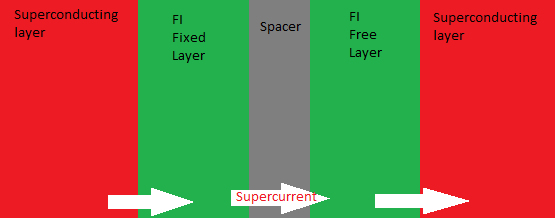
\includegraphics[width=12cm]{mtj}
    \caption{A very basic construction of an MTJ, consisting of a fixed(pinned) magnetisation layer, and free layer where magnetisation can be flipped via an external magnetic field.}
    \end{measuredfigure}
    \end{figure} 
    
JMRAM works on the principle of the Josephson effect\cite{josephson}. In this phenomenon, two superconductors, separated by a ferromagnetic insulating layer (referred to as FI from here onwards), can transmit (super)current. This is because the Cooper pair of electrons formed in the superconductor, tunnels through the ferromagnetic layer, but it does so in a particularly interesting way due to the environmental magnetic moment.

\subsection{Quantum Transport}

It is well known, due to BCS theory \cite{BCS} that electrons in certain materials, below some transition temperature, form bound state singlet Cooper pairs. The pairs can also exist in triplet pairs in more exotic cases such as the superfluidity of Helium-3, but in regular metals where electrons are bound by electron-phonon mediated interactions, Cooper singlet states are formed. The Ferromagnetic insulators (FI) in the MTJ act as what are known as ``Half-Metals" (HM) \cite{HM}, which split the density of states N(E) of majority and minority (up and down) spin carriers by the Zeeman shift as a result of the chosen direction of magnetic field as shown in figure 2. 
\begin{figure}[htp]
    \centering
    \begin{measuredfigure}
    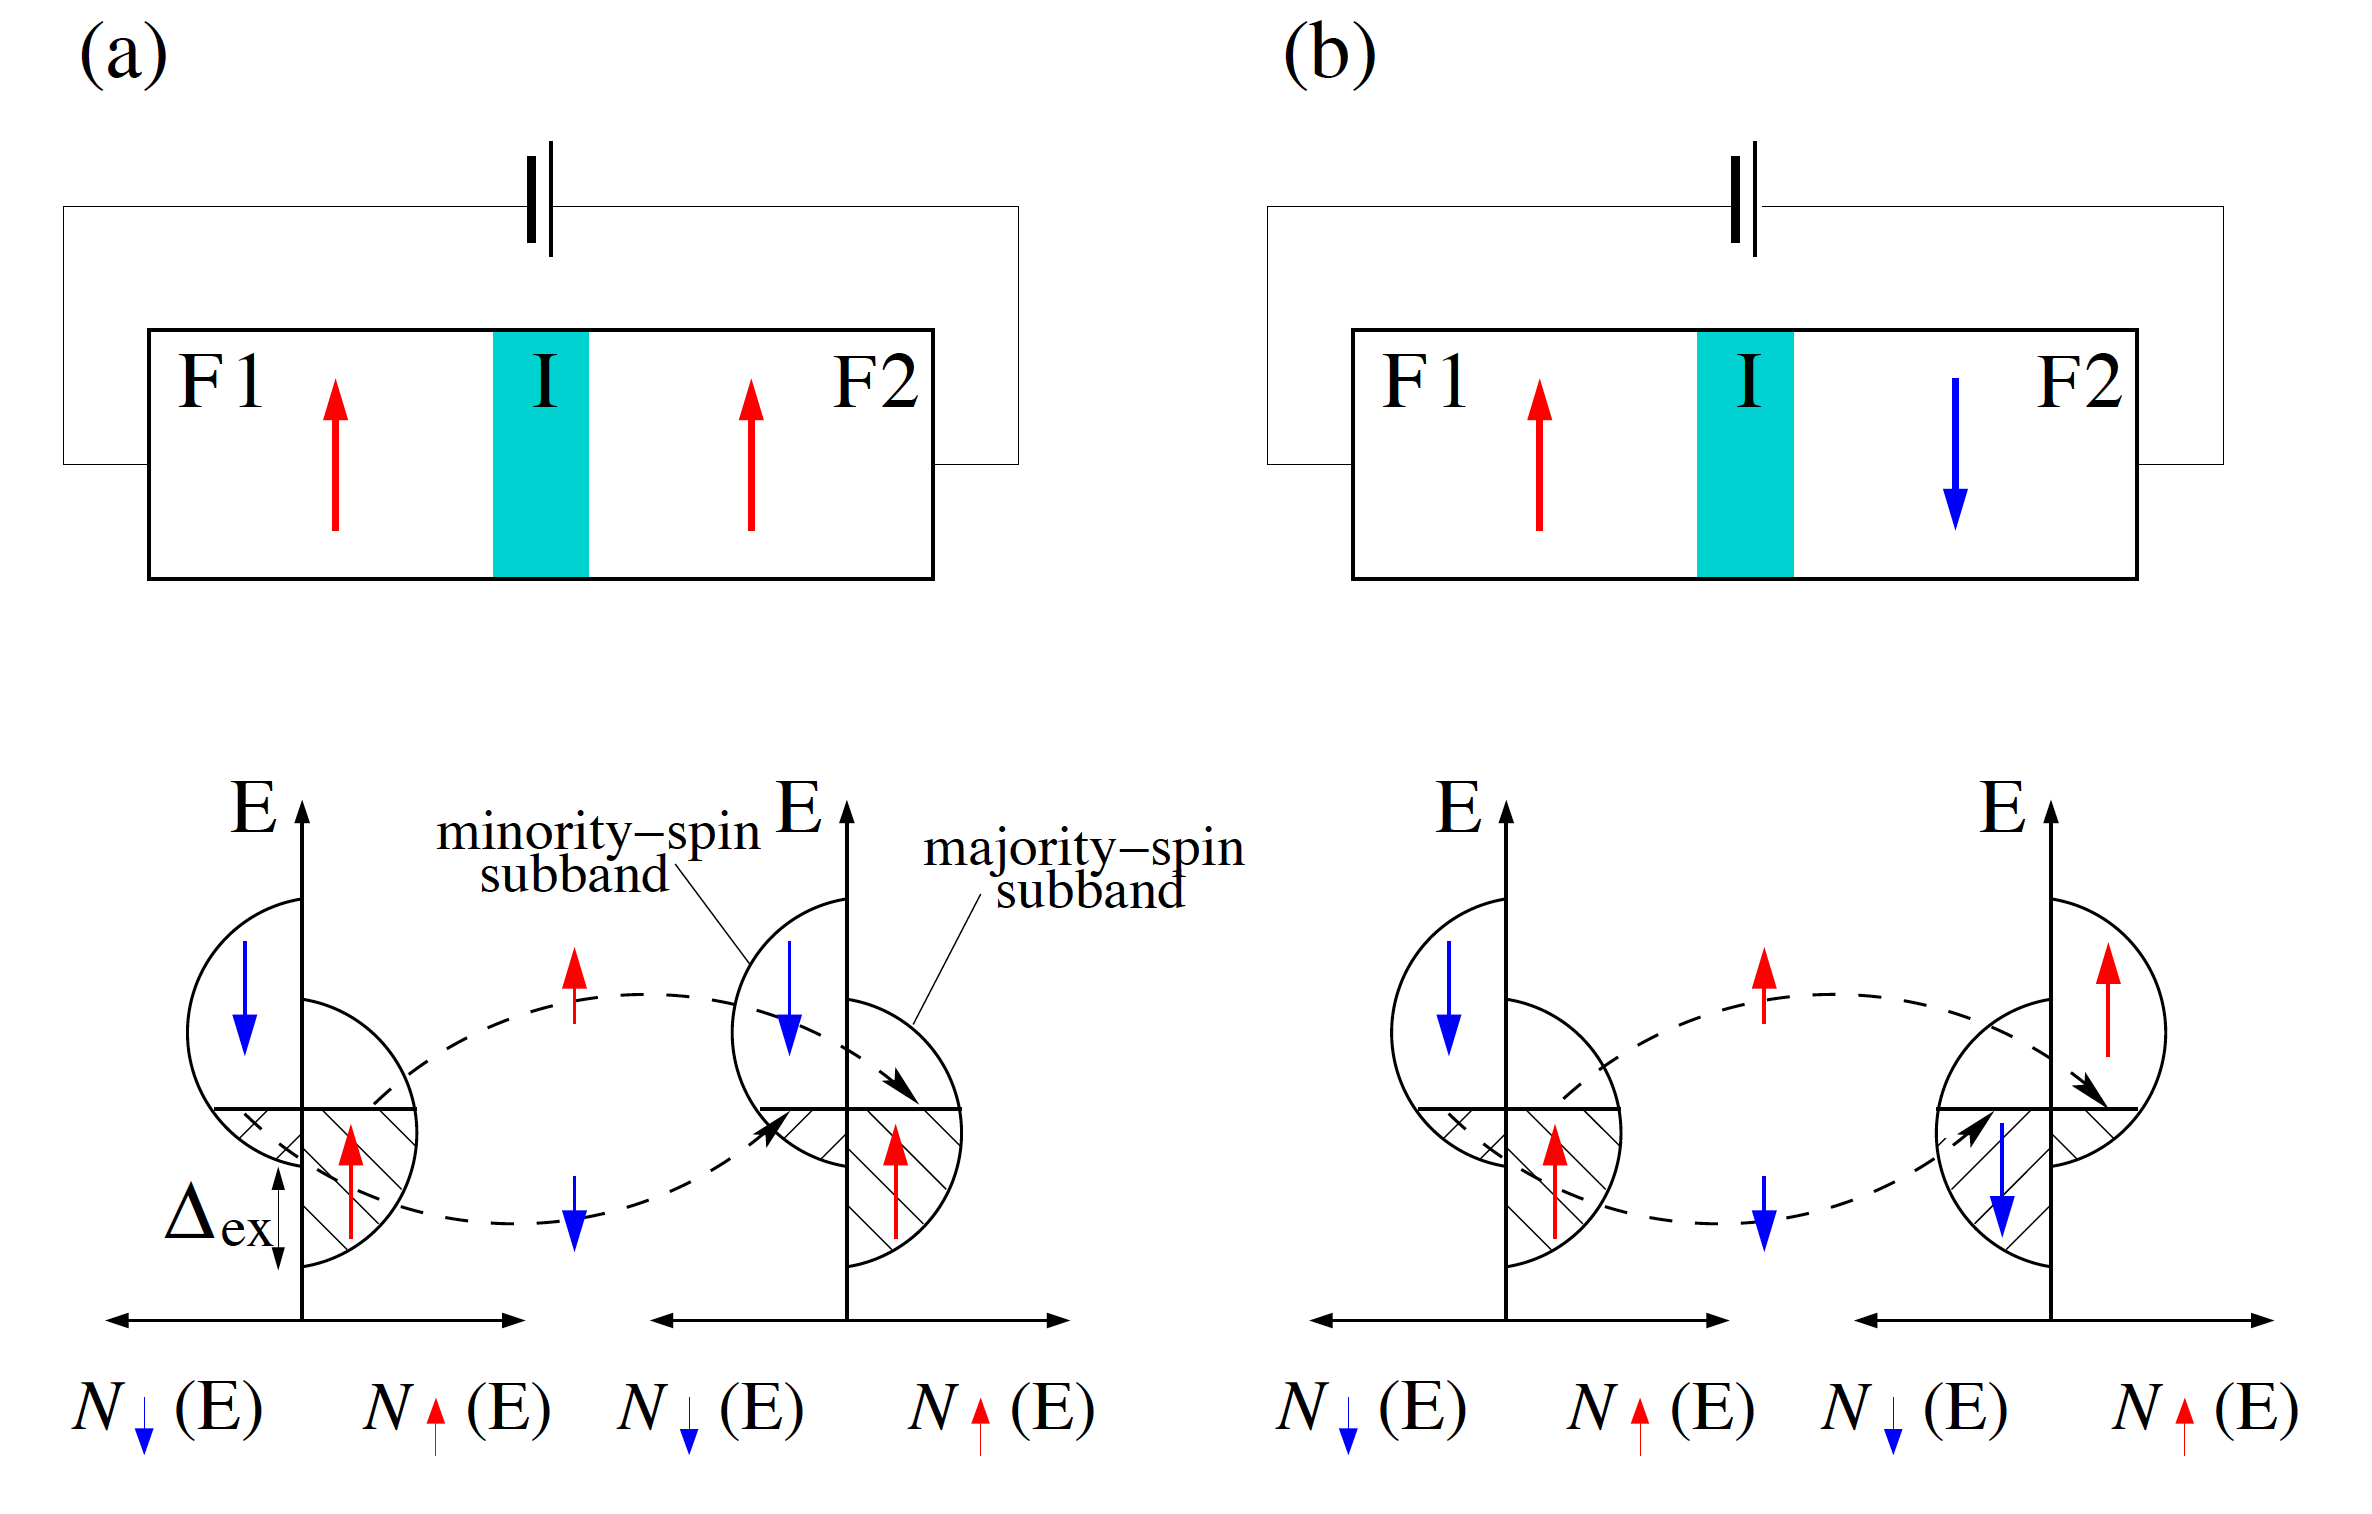
\includegraphics[width=10cm]{dos}
    \caption{Splitting of the majority and minority DOS N(E), due to the Zeeman effect, leading to tunnel magnetoresistance. Taken directly from \cite{fundapp}}
    \end{measuredfigure}
    \end{figure}
As a consequence of N(E) splitting, anti-parallel spin alignment between the superconducting electron (one of the pairs) and the FI magnetisation direction, results in an increase in the number of scattering channels, resulting therefore in increased magnetoresistance. By the same mechanism, parallel spin alignment results in a reduced magnetoresistance. It is this physical concept that is the heart of the MTJ. In this way, the Cooper pair could become unbound upon transmission to the FI layer. The electron with anti parallel spin quantisation direction to the ferromagnetic layer, would experience a Lorentz force. In this unstable state, the electron would like to align with the local environment's magnetic field. For Cooper pair transport through a superconductor-halfmetal\cite{HM} interface, the pair must "rotate" and pick up a phase, if it is to survive in the external magnetic field. The singlet pair is expressed as $\Psi=\frac{1}{\sqrt{2}}(\ket{\updownarrows}_{k,-k}- \ket{\downuparrows}_{k,-k}$, where the opposite electrons also have opposite but equal momentum (k,-k)\cite{BCS}. A phase difference upon reflectance must occur upon ferromagnetic layer transmission where $\ket{\uparrow}_{-k}=e^{i\theta/2}\ket{\uparrow}_k$ and $\ket{\downarrow}_{-k}=e^{-i\theta/2}\ket{\downarrow}_k$ \cite{contact}. Therefore the singlet state will now transform to
\begin{equation} \label{4.1} \tag{6.1}
\Psi=\frac{1}{\sqrt{2}}[e^{i\theta}\ket{\updownarrows}_{k,-k}- e^{-i\theta}\ket{\downuparrows}_{k,-k}]
\end{equation}

Now we see that the spin singlet can penetrate and survive the FI interface only if a phase difference $\theta$ occurs for the entire pair, and it rotates in the FI layer and forms a now "spin-mixed" singlet-triplet state. This is the Josephson effect for supercurrents \cite{josephson}. 
\begin{figure}[htp]
    \centering
    \begin{measuredfigure}
    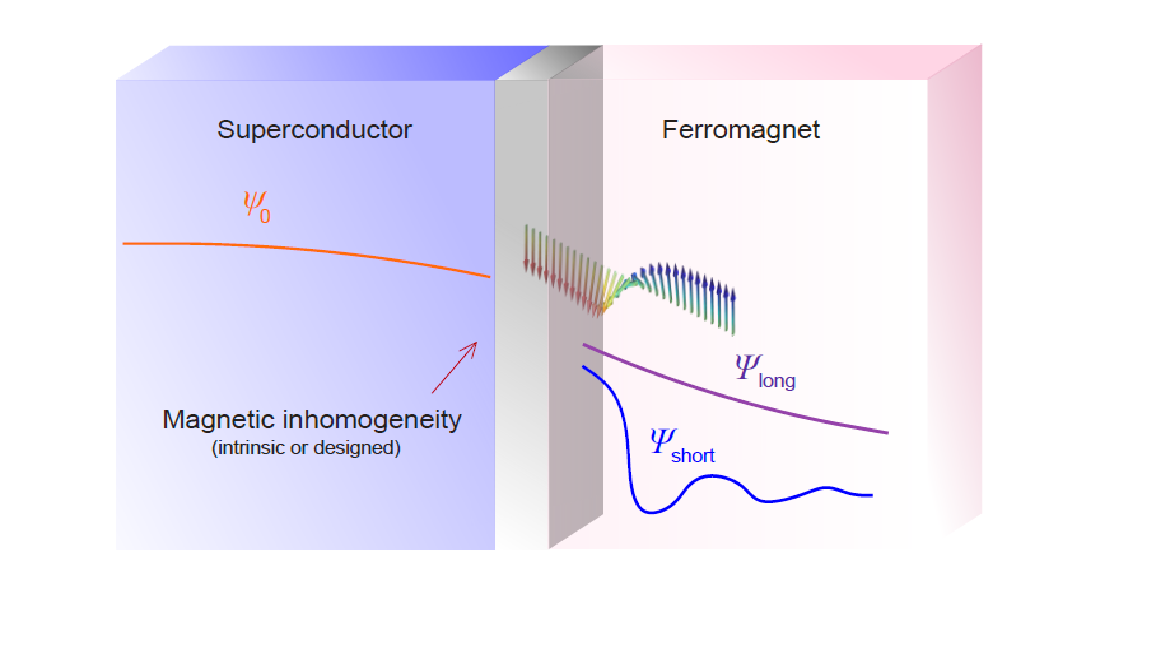
\includegraphics[width=15cm]{rot}
    \caption{The spin (intrinsic angular momentum) rotation of a particle upon transmission through the superconductor-ferromagnet interface where a magnetic field permeates.}
    \end{measuredfigure}
    \end{figure}

In combination with magnetoresistance, passing a supercurrent through the MTJ will result in a different resistance depending on the FI free layer's relative magnetisation quantisation axis to the fixed layer, providing the logic-state switching and valid application to transistors. Of course the FI thickness will affect phase difference at the end of the FI, so we choose a thickness that produces a $\Delta\theta=\pi$ (so called a pi-josephson junction). A more mathematically rigorous tight-binding treatment of cooper pair transport can be found in \cite{JMTJpi}, and yields a relationship between layer thickness and phase difference.

\subsection{The MTJ in question}


The MTJ that is being tested in this report, uses the superconducting material Niobium Nb. This has a transition temperature of about 9.3K, and since we require a reliable transistor, the running temperature should be in the range of about 4-5K. Figure 2 shows the construction of the JMRAM MTJ. The MTJ's FI layers must be alloys, specifically chosen to get rid of particular effects and amplify some others. The current tested FI is that of Permalloy (typically $Fe_{x}Ni_{1-x}$), alloyed with copper Cu. In the results chapter, it is found that the ideal permalloy configuration is roughly 20\% Iron and 80\% Nickel ($Fe_{20}Ni_{80}$), in keeping with standard and experimentally verified Permalloy results (\cite{permprob}).
\\
The free layer FI, must have low magnetostriction, that is to be able to switch magnetisation direction with a weak magnetic field, but of course not so weak that any background fields could affect the layer. The cause of the magnetostriction is anisotropy a magnetic material, causing it to easily magnetise in one direction but with more resistance in the other. Anisotropy can occur from complex spin-orbit coupling in the bulk (magnetocrystaline) and the physical dimensions of the material itself and how it is manufactured (shape). By choosing a material with low magnetocrystaline anisotropy, the shape anisotropy becomes the key factor in determining magnetostriction, which can be tuned, to construct a favourable MTJ. 
\\
Another factor is the spin lifetime through the layer, as impurities and defects may break the cooper pair. It has been found in (FIND PLS) that the lifetime $\tau$ is dependant on the inverse bandwidth(blurryness of spectral function) at a high symmetry point (usually X) at the Fermi energy E\textsubscript{F}. While this isn't quantitatively explored from the spectral data (discussed later), it is inferred from the band plots.
\\
We also wish to reduce the unfavorable scattering at the FI interface, which can be reduced by choosing a superconducting material with the same crystal structure and similar unit cell length to that of the FI layer. For instance Nb is BCC \cite{ashcroft} and Permalloy is FCC, so perhaps a better alloy ratio and choice is needed to create a more efficient MTJ. For example lead (Pb) is a BCS superconductor that has FCC crystal structure\cite{ashcroft} and a decent transition temperature of 7.19K. A band plot of the pure superconducting material will be compared to the spectral function of the random alloy to see how much they line up.

\subsection{Ferromagnetic Origins}

At the temperatures below the Curie temperature T\textsubscript{C}, the lattice spin sites, order and align in the same parallel direction, creating an overall macroscopic magnetic moment (magnetisation). The origin order arises from a quantum mechanical effect called the exchange interaction, and determines the T\textsubscript{C}. 
\\
Exchange interaction is not a force, but more of a bias towards having spins of the same spin to keep down the energy cost. Let us consider the singlet (s=0) and triplet (s=1) wavefunctions. The total Fermionic wavefunctions must be antisymmetric under particle exchange, giving rise to the following spatial and spinoral components of the wavefunction. Here the subscripts S and AS stand for symmetric and antisymmetric respectively (under particle exchange).
\begin{equation} \label{4.1} \tag{6.2}
\Psi_{singlet}(r_1,r_2)=\psi_{AS}\chi_S \qquad \Psi_{triplet}(r_1,r_2)=\psi_{S}\chi_{AS}
\end{equation}

The expected energies of the singlet (s=0) and triplet (s=1) states are

\begin{equation} \label{4.1} \tag{6.3}
E_s=\expval{H}_{singlet}=\int \Psi_s^*\hat{H}\Psi_sdr_1dr_2 \qquad E_t=\expval{H}_{triplet}=\int \Psi_t^*\hat{H}\Psi_tdr_1dr_2
\end{equation}



We know that from spin operator considerations that two coupled spins $S_1\cdot S_2$ have eigenvalues -3/4 and 1/4 for the singlet and triplet states respectively\cite{blundell} due to the following
$$\expval{2S_1\cdot S_2}=\bra{\Psi}S^2-S_1^2-S_2^2\ket{\Psi}=s(s+1)-2*\frac{3}{4}$$
Now the Hamiltonian for this simple 2 electron system can be written as
\begin{equation} \label{4.1} \tag{6.4}
\hat{H}=\frac{1}{4}(E_S-3E_T)-(E_S-E_T)\hat{S_1} \cdot \hat{S_2}
\end{equation}
The first term is a constant, but it is the spin interaction dependant term that is of interest.
We define the exchange parameter/constant J \cite{blundell}as
\begin{equation} \label{4.1} \tag{6.5}
J=\frac{E_S-E_T}{2}
\end{equation}

Now we have a spin-dependant Hamiltonian contribution of $H^{spin}=-2JS_1\cdot S_2$. From this simple 2 spin system we can generalise an approximation to describe a lattice of spins with each site labled i,j. Imposing that only exchange contribution from neighbouring sites, we obtain the Heisenberg model.
\begin{equation} \label{4.1} \tag{6.6}
H^{spin}=-\sum_{\expval{i,j}}J_{ij}S_i \cdot S_j
\end{equation}
\begin{equation} \label{4.1} \tag{6.7}
H=-\sum_{\expval{i,j}}J_{ij}S_i \cdot S_j-g\mu_BB\sum_iS_i
\end{equation}
Here g is the Landè g-factor, $\mu_B$ is the Bohr magneton and B is the magnetic field strength (which defines the z-direction). $J_{ij}$ is the exchange integral/parameter (6.5) between neighbouring spin sites on a lattice, i and j.
\\
Now we must link these exchange parameters J to the Curie temperature T\textsubscript{C}. We turn to mean field approximation methods to solve this problem. In this mean field, a spin at site i ($S_i$) experiences an average field of all spins surrounding it ($\expval{S_i}$). Realising $S_i=S_i-\expval{S_i}+\expval{S_i}$, one can expand to first order
$$S_i\cdot S_j=\expval{S_i}\expval{S_j}+\expval{S_i}(S_j-\expval{S_j}) + \expval{S_i}(S_i-\expval{S_i})$$

Plugging this back in to (6.7), one obtains the mean field Hamiltonian
\begin{equation} \label{4.1} \tag{6.8}
H_{mean-field}=\sum_{ij}J_{ij}\expval{S_i}\expval{S_j}-2\sum_{ij}J_{ij}S_i\cdot S_j--g\mu_BB_z\sum_iS^z_i
\end{equation}
Now let us consider the partition function for this system $Z=exp(-H/kT)$ where H is the mean field Hamiltonian, k is Boltzmann's constant and T is temperature. By appreciating that the magnetisation M(T) of the system is the mean field $\expval{S^z_i}$, one can (rather tediously) compute the magnetisation from a Brillouin function approach, and considering the point where magnetisation becomes non-zero. We assume that the choice of i and j is arbitrary such that $\expval{\hat{S_i}}=\expval{\hat{S_j}}$. We also chose a central point i=0, and define the exchange integral/constant as $J_0=\sum_jJ_{0j}$. Using the proof in \cite{meanfield}
one obtains $T_C=\frac{2(S+1)J_0}{3S}$ which in the classical limit of many spins as $S\rightarrow \infty $, reduces to
\begin{equation} \label{4.1} \tag{6.9}
T_C\approx\frac{2J_0}{3}
\end{equation}
The $J_0$ exchange parameter is essential in calculating the T\textsubscript{C}, and is an output of the 'lmgf' code as we shall see in the results section.
\clearpage
\section{Electronic Structure Calculations of FI layers}

\subsection{QUESTAAL suite}

The "Quasiparticle Electronic Structure and Augmented LMTO" (QUESTAAL) suite developed by Prof. Mark van Schilfgaarde and others \cite{ques}, has been used to obtain all subsequent results. The 'lmgf' code has been used extensively, implementing the theory of the previous chapters. The lmgf uses DFT and Green’s function formalism based on ASA-LMTO discussed previously. Bloch Spectral functions (electronic band structure for translationally invariant systems) can be calculated, and be read to see the effectiveness of the FI layer composition in electron transport. While the Green's function may contain less information than the full Hamiltonian, it allows for computation of many important results. It's ability to be configurationally averaged allows for the CPA implementation which is necessary for progression in alloy inspection. 'lmgf' also allows for calculation of magnetic exchange parameters, which determine the temperature condition necessary for transmission of spin waves through the FI layer(effectively Curie temperature). 
\\
As discussed in the JMRAM section, the superconducting layers are chosen to be Niobium (Nb), for it's high transition temperature. The FI layer composition, which is generally some appropriate deviation from Permalloy(Py), has been modified and tweaked in many different configurations to choose the most appropriate alloy for a JMRAM's MTJ. Many different quantities become important in alloy choice, and will now be expanded upon.

\subsection{Outline of procedure}

A ctrl input file must be constructed first with all relevant initial information about alloy composition, atomic numbers, etc.
The'lmstr' code is be used to calculate the structure constants necessary for ASA-LMTO (a very quick process). Then 'lmgf' must be used to calculate a self-consistent potential which usually takes a bit of time. Once a potential is found, the 'lmgf' switch --band:fn=syml uses self-consistent CPA to calculate the Omega Potential of CPA theory\cite{turek}.
\\Firstly, simulations of different Iron-Nickel alloy concentrations were investigated, and by observing the scattering in the spectral function plot, the best is chosen. To quench the magnetic moment, it is alloyed with copper by different amounts to see how much copper would be viable before there was too much scattering. A Curie temperature calculation was also carried out to test up to what temperature the alloy could retain a permanent magnetisation.
\\Then the procedure was repeated for an Iron-Chromium alloy, and again alloyed with copper. After this the last test is the compatibility of the superconductor-alloy interface. By plotting spectral functions of different superconductors, a quantitative comparison of alloy band structure was performed.

\subsection{Results}

Many different alloy configurations were tested for their effectiveness as FI layers. Bloch spectral functions must first be plotted for pure Permalloy ($Fe_{20}Ni_{80}$) and analysed. 
\begin{figure}[htp]
    \centering
    \begin{measuredfigure}
    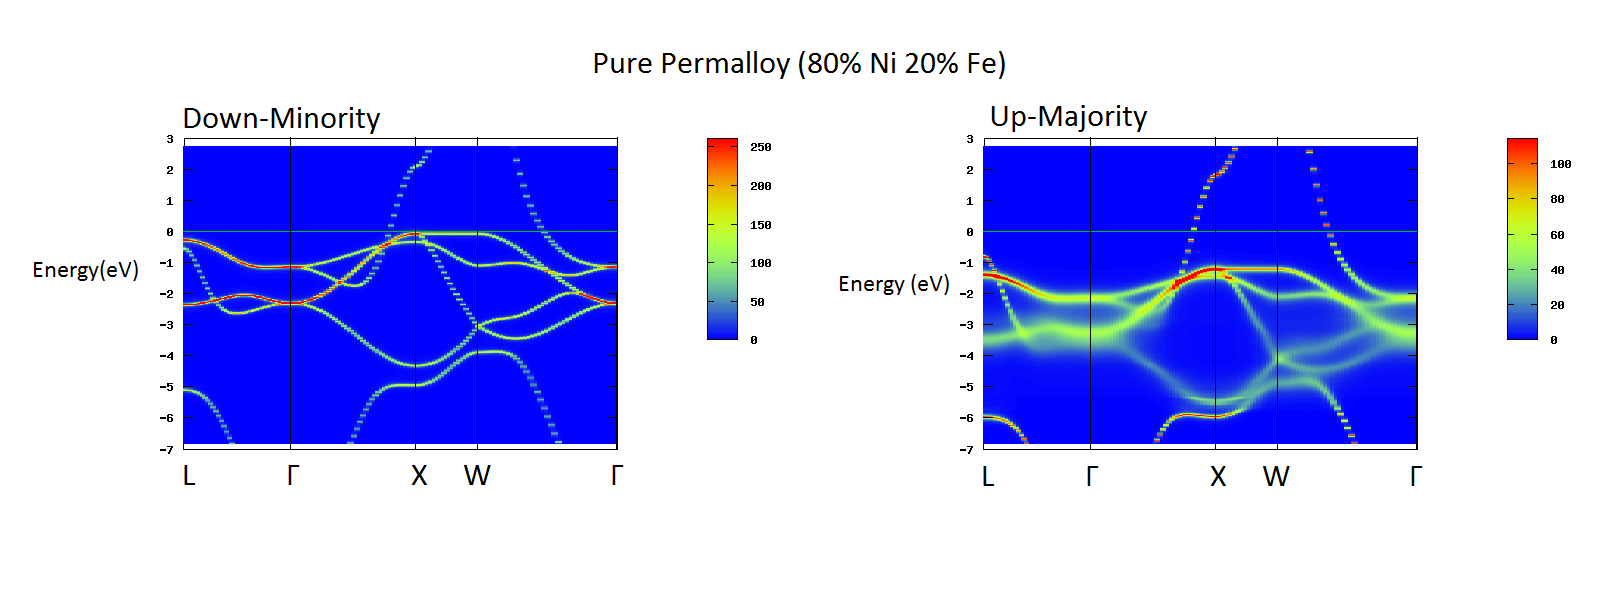
\includegraphics[scale=0.40]{specfunc/purepy}
    \caption{Plotted Bloch Spectral function for pure Permalloy $Py=Fe_{20}Ni_{80}$ via lmgf calculations}
    \end{measuredfigure}
    \end{figure}

Figure 4 shows that there is very little scattering (blurry/fuzziness) for the minority spin carriers, but more for the majority channel. Whilst we require both channels to have reduced scattering, this is ok. At first sight this seems like the perfect material for the MTJ, but the magnetic moment of the alloy must also be reduced. The reasoning for this is found in the JMRAM chapter. We wish to quench the magnetic moment by including a non-magnetic element into the alloy which will be copper Cu in this case. In other words to make the perfect MTJ, we wish to have a balance between low scattering, high spin lifetime, and low magnetisation. The addition of Cu to the alloy mix creates more scattering but quenches the magnetic moment, as can be seen in the following Spectral functions.

\begin{figure}[htp]
    \centering
    \begin{measuredfigure}
    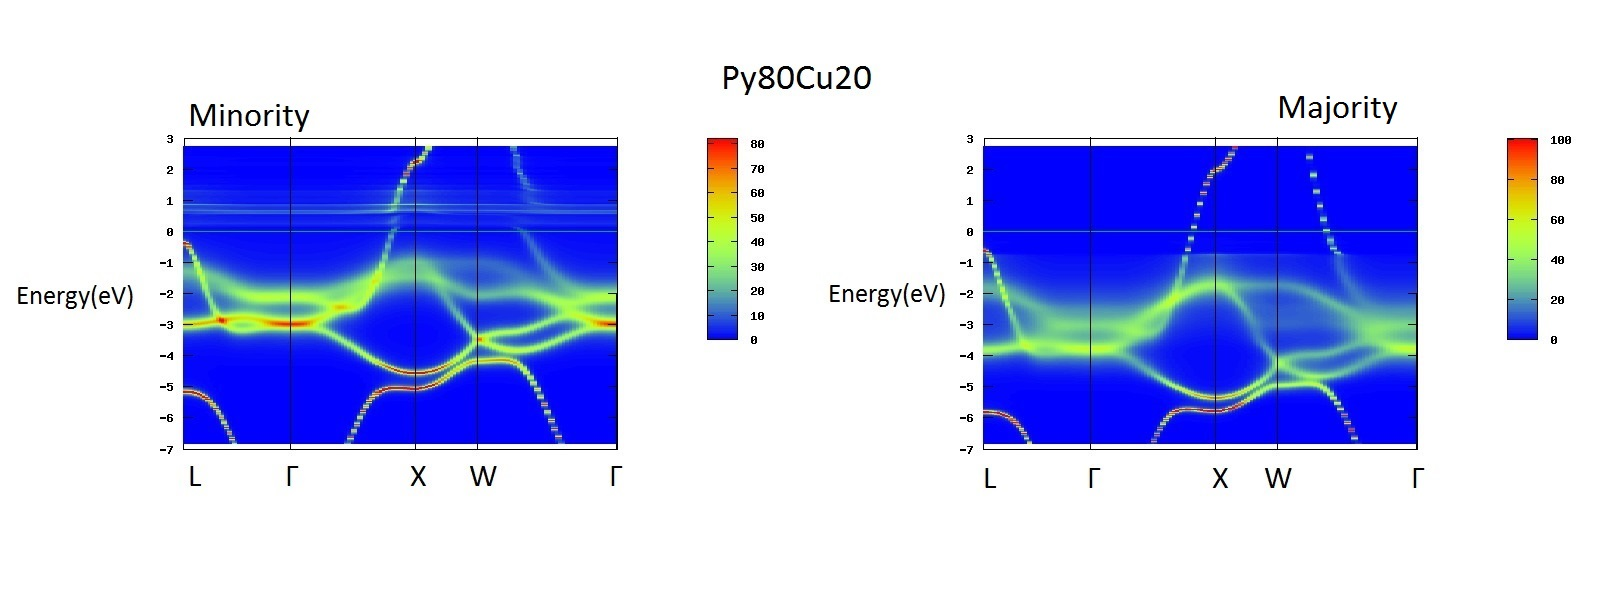
\includegraphics[scale=0.40]{specfunc/cu20}
    \caption{Plotted Bloch Spectral function for pure Permalloy $Py_{80}Cu_{20}$ via lmgf calculations}
    \end{measuredfigure}
    \end{figure}
\clearpage
Figure 5 shows that with just 20\% copper doping, scattering increases for both channels. The subsequent figures (6,7,8,9) also show the increased scattering through a higher Cu concentration. Interestingly the 80\Cu concentration shows relatively little scattering for both channels. This might be due to computational error.
\begin{figure}[h!]
    \centering
    \begin{measuredfigure}
    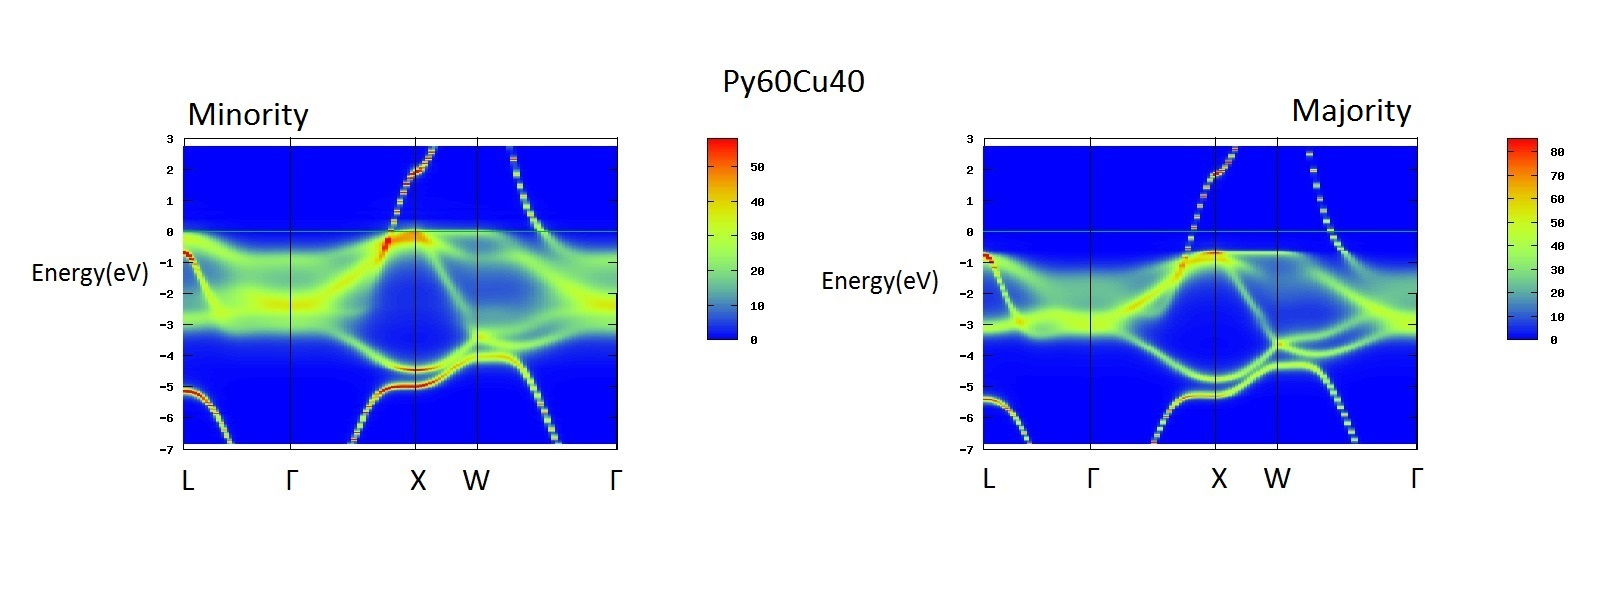
\includegraphics[scale=0.40]{specfunc/cu40}
    \caption{Plotted Bloch Spectral function for pure Permalloy-Copper alloy $Py_{60}Cu_{40}$ via lmgf calculations}
    \end{measuredfigure}
    \end{figure}
\begin{figure}[h!]
    \centering
    \begin{measuredfigure}
    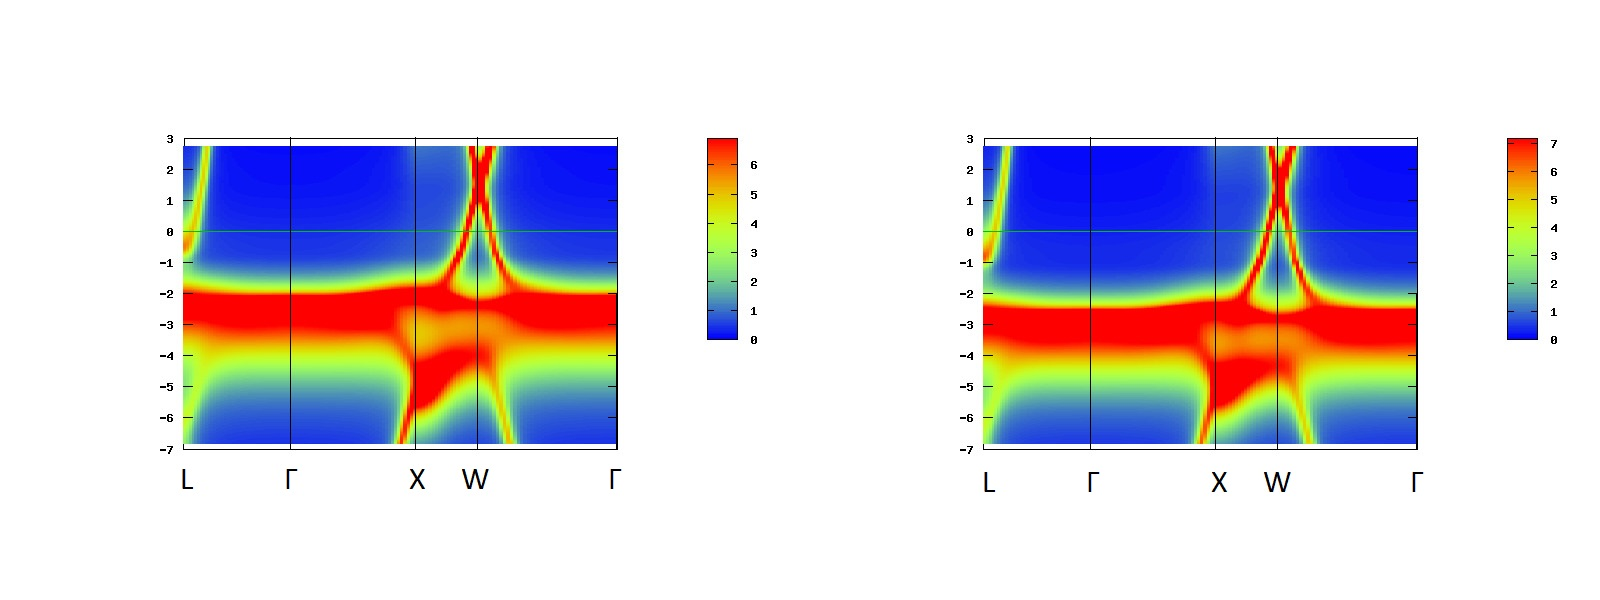
\includegraphics[scale=0.40]{specfunc/cu60}
    \caption{Plotted Bloch Spectral function for pure Permalloy-Copper alloy $Py_{40}Cu_{60}$ via lmgf calculations}
    \end{measuredfigure}
    \end{figure}
\begin{figure}[htp]
    \centering
    \begin{measuredfigure}
    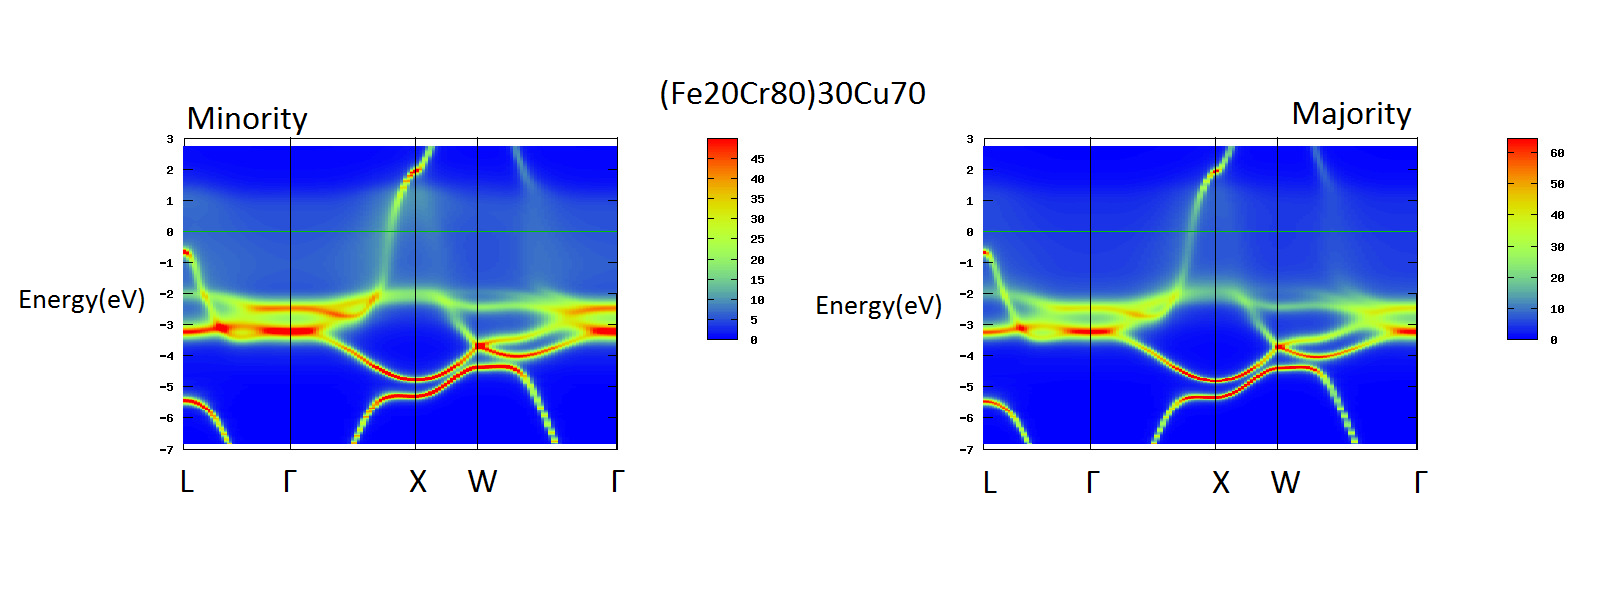
\includegraphics[scale=0.40]{specfunc/cu70}
    \caption{Plotted Bloch Spectral function for pure Permalloy-Copper alloy $Py_{30}Cu_{70}$ via lmgf calculations}
    \end{measuredfigure}
    \end{figure}
\begin{figure}[htp]
    \centering
    \begin{measuredfigure}
    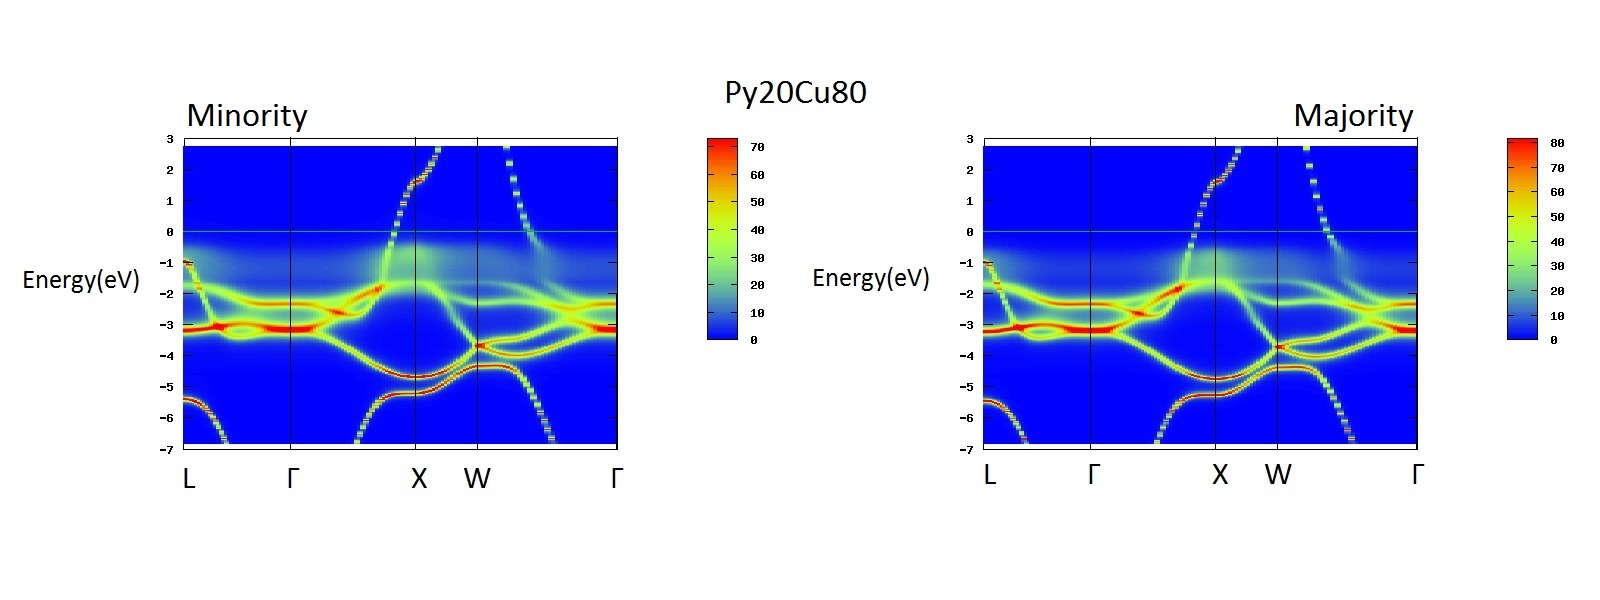
\includegraphics[scale=0.40]{specfunc/cu80}
    \caption{Plotted Bloch Spectral function for Permalloy-Copper alloy $Py_{20}Cu_{80}$ via lmgf calculations}
    \end{measuredfigure}
    \end{figure}
\clearpage
This ratio of Permalloy may not be ideal, so a simulation of ($Fe_{40}Ni_{60}$) was also carried out as shown in figure 10, but 



As is obvious, the spectral function of the different Permalloy ratio leads to a lot of scattering even before the introduction of any copper into the mix. For this reason, we keep the current ratio of Permalloy at ($Fe_{20}Ni_{80}$). But perhaps there is something else to do, what if the Nickel was replaced now with Chromium Cr. This choice is motivated by the Cr orbital structure, which is similar to Ni, as they are in the same row of the periodic table \cite{ashcroft}. However they differ in that pure Chromium forms in BCC structure with a lattice constant of 2.88{\AA} and Nickel in FCC with 3.52{\AA}. Their differences might produce better spectral functions, so first a test simulation of ($Fe_{99}Cr_{1}$) was carried out with doubts as to its ferromagnetic properties.

Firstly pure ($Fe_{20}Cr_{80}$) then addition of copper to quench again the magnetic moment. The following spectral functions show these results:



PUT IN

Now we consider the magnetic moments of all these different alloys in the following table, which are outuputs of the lmgf code.
\\ 
MAKE THIS
\\
\clearpage
Another factor to consider is the Curie temperature of all of these alloys to see if they are viable for running under the superconducting critical temperature of Niobium, and certainly ideally at about 4-5K. Exchange integrals/parameters $J_0$ (discussed earlier) are self consistently calculated for each element. A total $J_0$ can be calculated by considering the contribution from each element in the alloy. Then using the mean-field 2/3 law (6.8) , we can obtain the Curie temperature. Calculating the total $J_0$ was obtained by multiplying the individual exchange constants for each element. E.g. for $Py_{80}Cu_{20}=(Fe_{20}Ni_{80})_{80}Cu_{20}$, $J_0^{total}=J_0^{Fe}*0.2*0.8+J_0^{Ni}*0.8*0.8+J_0^{Cu}*0.2$. The units of mRy needed to be converted also to Joules J, by the conversion factor $1mRy=\frac{0.001*13.6}{0.00008617}J$.
\begin{table}[h!]
\centering
 \begin{tabular}{||c c c c c c||} 
 \hline
 Alloy Ratio & $J_0^{Fe}$ & $J_0^{Ni}$ & $J_0^{Cu}$ & $J_0^{Total}$ & Curie $T_C$ \\ [1ex] 
 \hline\hline
 $Py$ & 10.34 & 4.607 & null & 5.7536 & 605.38 \\ 
 $Py_{80}Cu_{20}$ & 8.662 & 2.509 & 0.096 & 3.01088 & 316.80 \\
 $Py_{60}Cu_{40}$ & 6.731 & 1.861 & 0.056 & 1.7234 & 181.33 \\
 $Py_{40}Cu_{60}$ & 5.297 & 1.148 & 0.022 & 0.80432 & 84.63 \\
 $Py_{20}Cu_{80}$ & 2.447 & 0.052 & 0.003 & 0.1086 & 11.43 \\ [1ex] 
 \hline
 \end{tabular}
\caption{The calculation of Curie temperature T\textsubscript{C}(K) from exchange constants J\textsubscript{0}(mRy), for different ratios of pure permalloy Py-$Fe_{20}Cr_{80}$ and copper Cu.} 
\end{table}

The overall magnetic moment of the materials was also calculated by 'lmgf', yielding the following table (2).

\begin{table}[h!]
\centering
 \begin{tabular}{||c c||} 
 \hline
 Alloy Ratio & Magnetisation[$emu/cm^3$] \\ [1ex] 
 \hline\hline
 $Py$ & 1144.67 \\ 
 $Py_{80}Cu_{20}$ & 615.49 \\
 $Py_{60}Cu_{40}$ & 445.70 \\
 $Py_{40}Cu_{60}$ & 277.08 \\
 $Py_{20}Cu_{80}$ & 89.76 \\ [1ex] 
 \hline
 \end{tabular}
\caption{The calculation magnetic moment for different ratios of pure permalloy Py-$Fe_{20}Ni_{80}$ and copper Cu, in units of $[emu/cm^3]$} 
\end{table}

\begin{table}[h!]
\centering
 \begin{tabular}{||c c||} 
 \hline
 Alloy Ratio & Magnetisation[$emu/cm^3$] \\ [1ex] 
 \hline\hline
 $Fe_{99}Cr_1$ & 1893.10\\ 
 $Fe_{90}Cr_{10}$ & 1627.15\\
 $Fe_{60}Cr_{40}$ & 964.56 \\
 $(Fe_{90}Cr_{10})_{90}Cu_{20}$ & 1316.01\\ 
 $(Fe_{90}Cr_{10})_{60}Cu_{40}$ & 1007.13\\  
 $(Fe_{90}Cr_{10})_{40}Cu_{60}$ & 664.71\\
 $(Fe_{60}Cr_{40})_{80}Cu_{20}$ & 774.99\\ [1ex]
 \hline
 \end{tabular}
\caption{The calculation magnetic moment for different ratios of pure permalloy Py-$Fe_{x}Cr_{1-x}$, in units of $[emu/cm^3]$} 
\end{table}

\begin{table}[h!]
\centering
 \begin{tabular}{||c c c c c c||} 
 \hline
 Alloy Ratio & $J_0^{Fe}$ & $J_0^{Cr}$ & $J_0^{Cu}$ & $J_0^{Total}$ & Curie $T_C$ \\ [1ex] 
 \hline\hline
 $Fe_{99}Cr_1$ & 12.369 & 15.346 & null & 12.399 & 1304.58 \\ 
 $Fe_{90}Cr_{10}$ & 12.358 & 6.98 & null & 11.820 & 1243.702\\
 $Fe_{60}Cr_{40}$ & 9.238 & 0.457 & null & 8.543 & 898.834 \\
 $(Fe_{90}Cr_{10})_{90}Cu_{20}$ & 11.020 & 7.487 & 0.046 & 8.543 & 898.834 \\ 
 $(Fe_{90}Cr_{10})_{60}Cu_{40}$ & 10.337 & 6.238 & 0.068 & 5.983 & 629.570 \\
 $(Fe_{90}Cr_{10})_{40}Cu_{60}$ & 8.835 & 3.518 & 0.077 & 3.368 & 354.325 \\ 
 $(Fe_{60}Cr_{40})_{80}Cu_{20}$ & 10.337 & 6.238 & 0.068 & 5.983 & 629.570 \\
 $(Fe_{60}Cr_{40})_{70}Cu_{30}$ & 10.337 & 6.238 & 0.068 & 5.983 & 629.570 \\
 $(Fe_{60}Cr_{40})_{60}Cu_{40}$ & 10.337 & 6.238 & 0.068 & 5.983 & 629.570 \\ [1ex]
 \hline
 \end{tabular}
\caption{The calculation of Curie temperature T\textsubscript{C}(K) from exchange constants J\textsubscript{0}(mRy), for different ratios of Iron-chromium alloy, and alloyed with copper Cu.} 
\end{table}

\section{Analysis and Conclusion}



\clearpage
\printbibliography




\end{document}
